%%%%%%%%%%%%%%%%%%%%%%%%%%%%%%%%%%%%%%%%%
% Masters/Doctoral Thesis
% LaTeX Template
% Version 2.5 (27/8/17)
%
% This template was downloaded from:
% http://www.LaTeXTemplates.com
%
% Version 2.x major modifications by:
% Vel (vel@latextemplates.com)
%
% This template is based on a template by:
% Steve Gunn (http://users.ecs.soton.ac.uk/srg/softwaretools/document/templates/)
% Sunil Patel (http://www.sunilpatel.co.uk/thesis-template/)
%
% Template license:
% CC BY-NC-SA 3.0 (http://creativecommons.org/licenses/by-nc-sa/3.0/)
%
%%%%%%%%%%%%%%%%%%%%%%%%%%%%%%%%%%%%%%%%%

%----------------------------------------------------------------------------------------
%	PACKAGES AND OTHER DOCUMENT CONFIGURATIONS
%----------------------------------------------------------------------------------------

\documentclass[
12pt, % The default document font size, options: 10pt, 11pt, 12pt
oneside, % Two side (alternating margins) for binding by default, uncomment to switch to one side
english, % ngerman for German
onehalfspacing, % Single line spacing, alternatives: onehalfspacing or doublespacing
%draft, % Uncomment to enable draft mode (no pictures, no links, overfull hboxes indicated)
%nolistspacing, % If the document is onehalfspacing or doublespacing, uncomment this to set spacing in lists to single
%liststotoc, % Uncomment to add the list of figures/tables/etc to the table of contents
%toctotoc, % Uncomment to add the main table of contents to the table of contents
%parskip, % Uncomment to add space between paragraphs
%nohyperref, % Uncomment to not load the hyperref package
headsepline, % Uncomment to get a line under the header
%chapterinoneline, % Uncomment to place the chapter title next to the number on one line
%consistentlayout, % Uncomment to change the layout of the declaration, abstract and acknowledgements pages to match the default layout
]{MastersDoctoralThesis} % The class file specifying the document structure

\usepackage[utf8]{inputenc} % Required for inputting international characters
\usepackage[T1]{fontenc} % Output font encoding for international characters
\usepackage{todonotes}
\usepackage{mathpazo} % Use the Palatino font by default

%\usepackage[style=numeric]{biblatex} % Use the bibtex backend with the authoryear citation style (which resembles APA)
\usepackage[backend=bibtex,style=numeric]{biblatex}
\bibliography{thesis, chapters/literature_review/literature_review, chapters/project_plan/project_plan}
\nocite{*}

\usepackage[autostyle=true]{csquotes} % Required to generate language-dependent quotes in the bibliography
\usepackage{multirow}
\usepackage{colortbl}
\usepackage{listings}
\usepackage{titlesec}
\titleformat{\chapter}{\huge\raggedright}{\MakeUppercase{\thechapter}}{1em}{}

\lstset{basicstyle=\ttfamily\footnotesize,breaklines=true}

%----------------------------------------------------------------------------------------
%	MARGIN SETTINGS
%----------------------------------------------------------------------------------------

\geometry{
	paper=a4paper, % Change to letterpaper for US letter
	inner=2.5cm, % Inner margin
	outer=3.8cm, % Outer margin
	bindingoffset=.5cm, % Binding offset
	top=1.5cm, % Top margin
	bottom=1.5cm, % Bottom margin
	%showframe, % Uncomment to show how the type block is set on the page
}

%----------------------------------------------------------------------------------------
%	THESIS INFORMATION
%----------------------------------------------------------------------------------------

% Your thesis title, this is used in the title and abstract, print it elsewhere with \ttitle
\thesistitle{Performance Augmentation using Biosignals}
% Your supervisor's name, this is used in the title page, print it elsewhere with \supname
\supervisor{Associate Professor Kenneth Pope}
% Your examiner's name, this is not currently used anywhere in the template, print it elsewhere with \examname
\examiner{}
% Your degree name, this is used in the title page and abstract, print it elsewhere with \degreename
\degree{Bachelor of Engineering (Electronics) (Honours)}
% Your name, this is used in the title page and abstract, print it elsewhere with \authorname
\author{Cooper Wolfden}
% Your address, this is not currently used anywhere in the template, print it elsewhere with \addressname
\addresses{}

% Your subject area, this is not currently used anywhere in the template, print it elsewhere with \subjectname
\subject{Electronic Engineering}
% Keywords for your thesis, this is not currently used anywhere in the template, print it elsewhere with \keywordnames
\keywords{Biosensors, Lighting control, Musical instrument digital interfaces, Wearable sensors}
% Your university's name and URL, this is used in the title page and abstract, print it elsewhere with \univname
\university{\href{https://www.flinders.edu.au/}{Flinders University}}
% Your department's name and URL, this is used in the title page and abstract, print it elsewhere with \deptname
\department{\href{https://www.flinders.edu.au/college-science-engineering}{College of Science and Engineering}}
% Your research group's name and URL, this is used in the title page, print it elsewhere with \groupname
\group{}
% Your faculty's name and URL, this is used in the title page and abstract, print it elsewhere with \facname
\faculty{\href{}{}}

\AtBeginDocument{
\hypersetup{pdftitle=\ttitle} % Set the PDF's title to your title
\hypersetup{pdfauthor=\authorname} % Set the PDF's author to your name
\hypersetup{pdfkeywords=\keywordnames} % Set the PDF's keywords to your keywords
}

\begin{document}

\frontmatter % Use roman page numbering style (i, ii, iii, iv...) for the pre-content pages

\pagestyle{plain} % Default to the plain heading style until the thesis style is called for the body content

%----------------------------------------------------------------------------------------
%	TITLE PAGE
%----------------------------------------------------------------------------------------

\begin{titlepage}
\begin{center}

\vspace*{.06\textheight}
{\scshape\LARGE \univname\par}\vspace{1.5cm} % University name
\textsc{\Large Honours Thesis}\\[0.5cm] % Thesis type

\HRule\\[0.4cm] % Horizontal line
{\huge \bfseries \ttitle\par}\vspace{0.4cm} % Thesis title
\HRule\\[1.5cm] % Horizontal line

\begin{minipage}[t]{0.4\textwidth}
\begin{flushleft} \large
\emph{Author:}\\
{\authorname} % Author name - remove the \href bracket to remove the link
\end{flushleft}
\end{minipage}
\begin{minipage}[t]{0.4\textwidth}
\begin{flushright} \large
\emph{Supervisor:} \\
{\supname} % Supervisor name - remove the \href bracket to remove the link
\end{flushright}
\end{minipage}\\[3cm]

\vfill

\large \textit{A thesis submitted in fulfillment of the requirements\\ for the degree of \degreename}\\[0.3cm] % University requirement text
%%\groupname\\\deptname\\[2cm] % Research group name and department name

\vfill

{\large October 16, 2023}\\[4cm] % Date
%\includegraphics{Logo} % University/department logo - uncomment to place it

\vfill
\end{center}
\end{titlepage}

%----------------------------------------------------------------------------------------
%	DECLARATION PAGE
%----------------------------------------------------------------------------------------

\begin{declaration}
\addchaptertocentry{\authorshipname} % Add the declaration to the table of contents
\noindent I, \authorname, declare that this thesis titled, \enquote{\ttitle} and the work presented in it are my own. I confirm that:

\begin{itemize}
\item This work was done wholly while in candidature for a degree of \degreename.
\item This document is in accordance with the plagiarism policy of \univname.
\item Where any part of this thesis has previously been submitted for a degree or any other qualification at this University or any other institution, this has been clearly stated.
\item Where I have consulted the published work of others, this is always clearly attributed.
\item Where I have quoted from the work of others, the source is always given. With the exception of such quotations, this thesis is entirely my own work.
\item I have acknowledged all main sources of help.
\item Where the thesis is based on work done by myself jointly with others, I have made clear exactly what was done by others and what I have contributed myself.\\
\end{itemize}

\noindent Signed:\\
\rule[0.5em]{25em}{0.5pt} % This prints a line for the signature

\noindent Date:\\
\rule[0.5em]{25em}{0.5pt} % This prints a line to write the date
\end{declaration}

\cleardoublepage

%----------------------------------------------------------------------------------------
%	QUOTATION PAGE
%----------------------------------------------------------------------------------------

%\vspace*{0.2\textheight}

%\noindent\enquote{\itshape One of the major problems encountered in time travel is not that of becoming your own father or mother. There is no problem in becoming your own father or mother that a broad-minded and well-adjusted family can't cope with. There is no problem with changing the course of history—the course of history does not change because it all fits together like a jigsaw. All the important changes have happened before the things they were supposed to change and it all sorts itself out in the end.

%The major problem is simply one of grammar, and the main work to consult in this matter is Dr. Dan Streetmentioner's Time Traveler's Handbook of 1001 Tense Formations. It will tell you, for instance, how to describe something that was about to happen to you in the past before you avoided it by time-jumping forward two days in order to avoid it. The event will be descibed differently according to whether you are talking about it from the standpoint of your own natural time, from a time in the further future, or a time in the further past and is futher complicated by the possibility of conducting conversations while you are actually traveling from one time to another with the intention of becoming your own mother or father.

%Most readers get as far as the Future Semiconditionally Modified Subinverted Plagal Past Subjunctive Intentional before giving up; and in fact in later aditions of the book all pages beyond this point have been left blank to save on printing costs.

%The Hitchhiker's Guide to the Galaxy skips lightly over this tangle of academic abstraction, pausing only to note that the term "Future Perfect" has been abandoned since it was discovered not to be.}\bigbreak

%\hfill The Hitch Hiker's Guide To The Galaxy

%----------------------------------------------------------------------------------------
%	ABSTRACT PAGE
%----------------------------------------------------------------------------------------

\begin{abstract}
  \addchaptertocentry{\abstractname} % Add the abstract to the table of contents

  This thesis aims to establish a platform for performers to utilize biological signals in order to create engaging live performances.
  This project is a continuation of the `Music from Biosignals' project, with the new addition of lighting control.

  The initial phase of the project began with the implementation of the lighting controller,
  enabling the system to interface with standard performance lighting fixtures.
  There are two parts of the lighting controller,
  an off-the-shelf controller, ensuring high reliability,
  and a prototyping fixture, allowing fast and cost-effective testing.
  These additions allow for the creation of exciting and engaging lighting patterns from collected biosensors.

  Further project developments involved the previously designed hardware,
  consisting of a PIC32 microcontroller, an ESP32 wireless transmitter, and an ADS1294R analog-to-digital converter.
  For this hardware, programming inconsistencies were resolved,
  over-the-air updates were implemented for the ESP32,
  and hardware debugging was enabled for the PIC32.

  Following this, consistent device-to-device communication was established.
  With successful communication between the PIC32 and ESP32 over SPI,
  challenges overcome with communication between the ADS1294R and PIC32,
  and the ESP32 acting as a wireless bridge with the off-body PC via TCP/IP.

  Despite these achievements, power issues during the final stage of development caused the device to fail in providing wireless sensor readings for the off-body PC to process.
  Thorough testing showed that the issue was related to the high impedance of the power plane.
  In conclusion, while the performance augmentation platform is not fully functional, significant strides have been made in resolving communication issues and establishing a foundation for future iterations.
  Recommendations for a second version include addressing power distribution challenges and optimizing overall current draw.
\end{abstract}

%----------------------------------------------------------------------------------------
%	ACKNOWLEDGEMENTS
%----------------------------------------------------------------------------------------

\begin{acknowledgements}
\addchaptertocentry{\acknowledgementname} % Add the acknowledgements to the table of contents
I would like to thank Craig Dawson for their professional advice and skills that helped immensely in the development of this project.
I would like to thank Associate Professor Kenneth Pope for their help in guiding me throughout this project and providing the much needed pressure when necessary.
Lastly, I would like to thank my friends and family for providing much needed relief from the various stresses of this year.
\end{acknowledgements}

%----------------------------------------------------------------------------------------
%	LIST OF CONTENTS/FIGURES/TABLES PAGES
%----------------------------------------------------------------------------------------

\tableofcontents % Prints the main table of contents

\listoffigures % Prints the list of figures

%\listoftables % Prints the list of tables

%----------------------------------------------------------------------------------------
%	ABBREVIATIONS
%----------------------------------------------------------------------------------------

%\begin{abbreviations}{ll} % Include a list of abbreviations (a table of two columns)

%\textbf{LAH} & \textbf{L}ist \textbf{A}bbreviations \textbf{H}ere\\
%\textbf{WSF} & \textbf{W}hat (it) \textbf{S}tands \textbf{F}or\\

%\end{abbreviations}

%----------------------------------------------------------------------------------------
%	PHYSICAL CONSTANTS/OTHER DEFINITIONS
%----------------------------------------------------------------------------------------

%\begin{constants}{lr@{${}={}$}l} % The list of physical constants is a three column table

% The \SI{}{} command is provided by the siunitx package, see its documentation for instructions on how to use it

%Speed of Light & $c_{0}$ & \SI{2.99792458e8}{\meter\per\second} (exact)\\
%Constant Name & $Symbol$ & $Constant Value$ with units\\

%\end{constants}

%----------------------------------------------------------------------------------------
%	SYMBOLS
%----------------------------------------------------------------------------------------

%\begin{symbols}{lll} % Include a list of Symbols (a three column table)

%$a$ & distance & \si{\meter} \\
%$P$ & power & \si{\watt} (\si{\joule\per\second}) \\
%Symbol & Name & Unit \\

%\addlinespace % Gap to separate the Roman symbols from the Greek

%$\omega$ & angular frequency & \si{\radian} \\

%\end{symbols}

%----------------------------------------------------------------------------------------
%	DEDICATION
%----------------------------------------------------------------------------------------

%\dedicatory{For/Dedicated to/To my\ldots}

%----------------------------------------------------------------------------------------
%	THESIS CONTENT - CHAPTERS
%----------------------------------------------------------------------------------------

\mainmatter % Begin numeric (1,2,3...) page numbering

\pagestyle{thesis} % Return the page headers back to the "thesis" style

% Include the chapters of the thesis as separate files from the Chapters folder
% Uncomment the lines as you write the chapters

\chapter{Introduction}
This project proposes the use of biosignals, such as heart rate and muscle movement, to augment performances by generating correlated music and lighting.
For instance, a person could perform a movement routine and have the music of that routine be generated in response to their movement,
as opposed to learning a routine based on a preexisting piece of musical composition.
Similarly, lighting could be used to enhance a performance by allowing audiences to have a visual representation of the inner working of a performer's body,
and how that changes based on the state of the performance and the response of the audience.
This opens up room for future exploration into how performance can change when specific movements have additional audio and visual elements,
and how different movements may be endowed with novel meaning from these additions.

\section{Background}
A biosignal is a form of communication between biological systems~\cite{semmlow:2018},
they are used in the body to detect various biological events such as muscle contractions and heartbeats~\cite{escabí:2012}.
These signals can be detected using various types of sensors, including electric, mechanical, acoustic, and infrared sensors~\cite{kaniusas:2012}.

Music has been a form of human expression for over 40,000 years~\cite{killin:2018}.
In recent times in western musical expression, the creation of music has relied on the skill and dexterity of artists
who have dedicated years to practicing in order to become proficient.
This has presented accessibility challenges for individuals who may be unable to physically perform such actions
or to those who do not have the time required to learn.
This project offers a solution to this challenge by providing a platform for creating music that can be accessible to everyone.
Additionally, this project allows for multifaceted performances due to the lack of physical restrictions on performers
during the dynamic creation of music.

This project is also beneficial to current artists as the addition of lighting control allows for more engaging performances.
Traditionally, lighting control is operated manually by a skilled lighting technician or automatically triggered by sound.
This project allows the lighting to be controlled directly by the performer, which could allow for much more compelling lighting setups.

\section{Aims}
The aims of this project are to create a software and hardware platform that can:

\begin{itemize}
        \item Control music and lighting in real-time from biosignals.
        \item Operate effectively in live performance spaces.
        \item Be wearable by a performer for an extended period of time without causing physical distress.
\end{itemize}

\section{Literature Review}
\subsection{Introduction}
The use of biosignals to generate music and lighting has been an area of exploration and innovation in the field of live performance technology.
In this literature review, we will examine various approaches and technologies that have been developed in the pursuit of creating music and lighting from biosignals.
We will begin by discussing early attempts at generating music from brainwaves,
and the challenges associated with using electroencephalogram (EEG) signals for live performances.
Then, we will explore the use of other biosignals such as electrocardiogram (ECG), electromyography (EMG), galvanic skin response (GSR), and respiratory rate,
which offer more predictability and discuss why they are better suited to this project.
Finally, we will investigate wireless solutions that enable the integration of biosensors into live performance devices,
and look into existing biosignal based lighting systems, before delving into the Music from Biosignals project;
a project that aims to incorporate biosignals into a wireless platform for live performance.
By reviewing these advancements, we hope to gain insights into the current state of the field and identify areas for further improvement and development.

% SHOULD GO INTO EVERY TYPE OF BIOSIGNAL AND THEN ARRIVE AT THESE SPECIFICALLY
% ALSO SHOULD NOT NECESARILLY ONLY LOOK AT MUSIC/PERFORMANCE FROM THEM
% SHOULD START MUCH WIDER AND THEN ARRIVE WHERE I STARTED HERE

\subsection{Music from Brainwaves}
The earliest attempt at creating music from brain activity is Alvin Lucier's `Music For Solo Performer'~\cite{Lucier:2010}\cite{Straebel:2014}.
While this system suffers from various technical issues such as high noise,
the fundamental issue with trying to use electroencephalogram (EEG) to generate any kind of performance signal
is that the output of an EEG is not at all rhythmic and contains a lot of randomness.
Additionally, EEG signals have a high potential for artifacting~\cite{Mannan:2018} and require a large number of electrodes~\cite{Piorecky:2019}.
These factors make EEG signals unsuitable for performance in a live setting and thus they will not be incorporated into the project.

\subsection{Rhythmic Signal Approach}
Other biosignals that could be used are electrocardiograms (ECG)~\cite{Afonso:1999}\cite{Pan:1985},
which is a common and painless measurement that is used to monitor the heart~\cite{Mayo:2023}.
Electromyography (EMG)~\cite{Tanaka:2002}\cite{Young:2013},
which measures electrical activity due to the response of muscles~\cite{Hopkins:2023}.
Galvanic skin response (GSR)~\cite{Kurniawan:2013},
which can show the intensity of emotional changes due to the change in conductance of the skin~\cite{Farnsworth:2018}.
And respiratory rate~\cite{Carlos:2011},
which measures the number of breaths per minute~\cite{Hopkins2:2023}.
These signals have a degree of predictability~\cite{Tahiroğlu:2008} which makes them better suited for use in this project.
There are a number of examples of these kinds of signals being incorporated into live performance settings such as
the `Conductor's Jacket' by Nakra and Picard~\cite{Nakra:1998}, and `Stethophone' by Nerness and Fuloria~\cite{Nerness:2019}.
However, these applications are still limited in their flexibility and use due to the restrictive wired nature of these devices.

% WIRELESS SOLUTION SHOULD COVER ALL KINDS OF WIRELESS TRANSMISSION
% RATHER THAN JUST WHAT HAS BEEN DONE IN THE BIOSIGNALS SPACE

\subsection{Wireless Solutions}
Wireless biosensor based performance devices do exist, but there is limited information on them.
Examples of such systems are Yamaha AI's `Transforms a Dancer into a Pianist'~\cite{Yamaha:2018}, and `Emovere' by Jaimovich~\cite{Jaimovich:2016}.
These systems allow performers to elevate their performances by adding an experimental aspect.
However, further exploration could still be done in this space with the addition of lighting control.

\subsection{Biosignal-based Lighting Control}
There is limited activity in controlling lighting using biosignals.
The most relevant research available is Wang's EMG-based Interactive Control Scheme for Stage Lighting~\cite{Wang:2022}.
This project uses EMG signals to control lighting in a live performance environment.
However, this project focuses on providing specific control of stage lighting using gestures.
For these gestures to work, the feature extraction algorithm of the device needs to be aware of specific gestures, which are predetermined by the developer.
This limits possible areas of creative exploration, as lighting compositions are predetermined rather than being `found' by the performer.
Thus, there is still room for further developments in this area.

\subsection{The Music from Biosignals Project}
The music from biosignals project has been an ongoing project that attempts to develop and integrate these previously mentioned gaps in literature.
The project has developed an on-body device that acquires biosensors and allows them to be wirelessly transmitted to a PC for processing~\cite{Pierro:2019}\cite{Tran:2022}.
Additionally, software developed in MATLAB has been developed that processes the incoming signals and generates music in real-time~\cite{Chen:2016}\cite{Nicholls:2019}.
Prior to the work set out in this thesis, the hardware and software elements of this project had been separate and not yet integrated.
This leaves potential future work open in connecting both sides of the project to create one cohesive whole.
Additionally, there has only ever been a musical aspect to the project, allowing further exploration into how lighting could improve the system.

\subsection{Conclusion}
In conclusion, the exploration of generating music from biosignals has seen significant progress in recent years.
While early attempts using brainwaves faced challenges due to their non-rhythmic and unpredictable nature,
other biosignals such as ECG, EMG, GSR, and respiratory rate have shown promise in generating more predictable and rhythmic signals for use in live performance environments.
While a number of projects have incorporated these signals, there is still room in the literature for exploration in applying these signals to lighting systems, in a way that does not limit the creativity of the performer.

\section{Project Plan}
\subsection{Project Objectives}
For this project to be successful, it is necessary to fulfill various requirements.
The requirements for this project are:

% TODO: THIS LIST SUCKS NEED TO DO IT BETTER
\begin{enumerate}
    \item The system must be composed of inexpensive parts
    \begin{enumerate}
        \item Sensors must fall within the allocated budget
        \item PCBs must use off the shelf, easily sourced components
        \item Components must be easily replaceable for minimal cost if something were to fail
    \end{enumerate}
    \item The system output must operate remotely to the acquired sensor data at a range of at least 30m
    \begin{enumerate}
        \item The acquisition of sensor data must be completely detached from the system output
        to allow for more complicated off-body setups
        \item The remote system must be compliant with ISO/IEC 15149-1:2014 or equivalent
        \item The wireless system must have a Packet Error Rate (PER) of no more than 1\%
        \item The wireless system must still be functional in a noisy environment
    \end{enumerate}
    \item The system must output MIDI messages
    \begin{enumerate}
        \item The MIDI output port must be IEC 63035:2017 compliant
        \item The system must also provide MIDI over USB for greater compatibility with newer devices
    \end{enumerate}
    \item The system must incorporate lighting control
\end{enumerate}

\subsection{Assumptions and Constraints}
Assumptions:
\begin{itemize}
    \item The system will be used in an indoor environment with stable temperature and humidity.
    \item The performers will be able to wear biosignal sensors comfortably during their performance.
    \item The sweat from the performers will be mitigated to avoid short-circuiting the electrodes.
    \item The system will exist in a stable performative enviroment.
        \begin{itemize}
                \item The various audio visual elements of the performative enviroment are functional.
                \item The system is being operated by skilled and knowledgable professionals.
        \end{itemize}
\end{itemize}

Constraints:
\begin{itemize}
    \item The total cost of the system cannot exceed \$600.
    \item The size and weight of the whole system must be compact enough to transport in a standard travel bag.
        \begin{itemize}
                \item The system must weigh less than 20kg.
                \item The system must take up less than 50L.
        \end{itemize}
    \item The size and weight of the on-body subsystem must be wearable for several hours without fatigue.
        \begin{itemize}
                \item The on-body element of the system must weigh less than 5kg.
        \end{itemize}
    \item The system must be compatible with a standard lighting protocol.
\end{itemize}

\subsection{Previous Work}
This project is a continuation of the Music from Biosignals project.
As such, a number of these objectives have already been fulfilled, and some hardware and software has been developed.
The extent of these developments are as follows:

\begin{itemize}
        \item Hardware for an on-body device has been developed.
        \begin{itemize}
                \item The hardware has been successfully powered on.
                \item Programmer communication with the microcontrollers has been established.
                \item One of the microcontrollers has been connected to WiFi.
        \end{itemize}
        \item Software for the off-body PC has been written.
        \begin{itemize}
                \item a MATLAB script that generates music using a prerecorded ECG biosignal has been developed.
        \end{itemize}
\end{itemize}

\subsection{Scope}
Given this project outline and the previous project work.
The scope of the project can be defined in~\autoref{tab:scope},~\autoref{tab:scope_stretch}, and~\autoref{tab:scope_out}.
This scope contains stretch goals because some of the previous work had not been completed at the start of the project,
as those students were finishing mid-year.
Therefore, the strech goals exist to allow the necessary project flexibility to account for various outcomes of those student's projects.

\begin{table}[!ht]
    \caption{Project in-scope list}\label{tab:scope}
    \centering
        \begin{tabular}{|l|c|}
        \hline
        \multirow{2}{7em}{On-body Device}     & \cellcolor{green!25}Communication between sub-systems           \\ \cline{2-2}
        ~                                     & \cellcolor{green!25}Basic sensor reading                        \\ \hline \hline
        \multirow{2}{7em}{Lighting Control}   & \cellcolor{green!25}Lighting fixture control                    \\ \cline{2-2}
        ~                                     & \cellcolor{green!25}Test setup                                  \\ \hline \hline
        \multirow{3}{7em}{System Integration} & \cellcolor{green!25}Wireless communication                      \\ \cline{2-2}
        ~                                     & \cellcolor{green!25}Integration with music generation           \\ \cline{2-2}
        ~                                     & \cellcolor{green!25}Integration with lighting generation        \\ \hline
    \end{tabular}

\end{table}

\begin{table}[!ht]
    \caption{Project stretch-goal list}\label{tab:scope_stretch}
    \centering
        \begin{tabular}{|l|c|}
        \hline
        Sensors                               & \cellcolor{orange!25}Wearable sensor design             \\ \hline \hline
        \multirow{3}{7em}{MIDI}               & \cellcolor{orange!25}Compliant MIDI implementation      \\ \cline{2-2}
        ~                                     & \cellcolor{orange!25}MIDI timecode quantisation         \\ \cline{2-2}
        ~                                     & \cellcolor{orange!25}MIDI output timecode               \\ \hline \hline
        \multirow{4}{7em}{System Integration} & \cellcolor{orange!25}Performance application testing    \\ \cline{2-2}
        ~                                     & \cellcolor{orange!25}Bi-directional communication       \\ \cline{2-2}
        ~                                     & \cellcolor{orange!25}Real-time system tunability        \\ \cline{2-2}
        ~                                     & \cellcolor{orange!25}PCB housing design for main board  \\ \hline
    \end{tabular}

\end{table}

\begin{table}[!ht]
    \caption{Project out-of-scope list}\label{tab:scope_out}
    \centering
        \begin{tabular}{|l|c|}
        \hline
        Sensors                               & \cellcolor{red!25}Sensors as independent systems        \\ \hline \hline
        \multirow{2}{7em}{MIDI}               & \cellcolor{red!25}Wireless MIDI                         \\ \cline{2-2}
        ~                                     & \cellcolor{red!25}MIDI threshold points                 \\ \hline \hline
        Lighting Control                      & \cellcolor{red!25}Lighting controller input support     \\ \hline \hline
        \multirow{2}{7em}{System Integration} & \cellcolor{red!25}Cableless system                      \\ \cline{2-2}
        ~                                     & \cellcolor{red!25}User interface for configuration      \\ \hline
    \end{tabular}

\end{table}

\chapter{Lighting Controller}
\section{Prototyping Fixture}
Small number of LEDs to verify correct control.
8 NeoPixel LEDs with 4 `dummy' DMX channels each.
DMX channels are intensity, red channel, green channel, blue channel.
Total of 32 channels (\(4 \times 8\))

\subsection{DMX}
Fixture uses Arduino along with
\href{https://github.com/mathertel/DMXSerial}DMXSerial library.
Receives DMX frames using interrupts
and stores them into array for processing.
DMX frames are 512 bytes wide.
A frame consists of the entire DMX `universe' of channels.
Individual channels are never written,
instead the entire `universe' is updated with each frame.
Updates happen continually at a known rate.
This way, fixture are aware if they lose connection to the controller,
since they stop receiving frames.

\subsection{NeoPixels}
LEDs controlled using \href{https://github.com/adafruit/Adafruit_NeoPixel}NeoPixel library.
LEDs can be colored independently using red, green, and blue values.
Each color is represented using a byte.

\subsection{Integration}
Both the DMX channel and color values are represented using bytes.
No additional scaling is required.

Brightness needs to be mapped using
\begin{lstlisting}[language=C]
  (intensity * color) >> 8;
\end{lstlisting}

In this case bit shifting by 8 is equivalent to dividing by 255.
This means that at maximum intensity the result of this calculation is the color value.
While at the minimum intensity the calculation becomes 0.

The values are sent over serial using Base64.
This is so that the carrige return line can be used to mark the end of the incoming values.
This was because the Arduino could become out of sync with what was being sent.
If this happened there is no way of getting back in sync,
because any special character could be interpreted as a regular value.
This is why Base64 is necessary, because it allows for special characters that are seperate
from the designated regular character set.
The values are sent as single decimal digits.
So when they are received they must be decoded back into bytes.

The value of each LED is then encoded across 4 bytes.
So the main program loops, incrementing by 4 each time,
and extracts the discrete bytes, setting the base address of the LED to the derived color.
Once this is done for all the LEDs, they are updated using the show() function.

\section{OpenDMX Controller}
When using expensive hardware in professional settings, it is important to use compliant hardware.
While the prototyping fixture could be used for system verification,
it was decided that existing hardware would be purchased for lighting control.
\textbf{DECISION MATRIX HERE (MIGHT ALREADY HAVE ONE IN MY RESULTS POWER POINT?)}

\subsection{Interface}
The driver provided by the manufacturer was written in C\#.
Existing code for the project is written in MATLAB.
We needed some way of controlling the device from MATLAB to utilise previous code.
\textbf{MORE TO BE WRITTEN ABOUT THIS}

\chapter{On-Body Device}
The on-body device was developed by William Tran in 2022~\cite{Tran:2022} and consists of two microcontrollers,
a PIC32 and a ESP32, as well as 24-bit ADC for taking biosignal measurements.

At the middle of the year when the project was handed over,
the ESP32 had been programmed to connect to WiFi, but was only programming intermittently,
and the PIC32 had bare-bones programming on it to enable the ESP32 via its enable pin.

The only other contributions were from Craig Dawson who supplied information and code for programming the PIC32,
as well as attaching wires to specific pins of the PIC32, allowing it to be probed using an oscilloscope.


\section{ESP32}
The ESP32 on the board is the ESP32-WROOM-32D.
This device is used as a wireless bridge between the on-body device and the off-body PC.
It connects to the PIC32 through a Serial Peripheral Interface (SPI) bus.
It is programmed using the Arduino software environment.

\subsection{Power}
As stated, the ESP32 was only programming intermittently.
To determine what the cause of this unwanted behavior was,
the board was tested in the following states in order to measure changes in how the ESP32 programmed.

\begin{itemize}
        \item The board was connected to a lab bench power supply with a non-restrictive current limit.
        \item The boot select switch was held for the extent of the programming cycle.
        \item The boot select switch was held until programming began.
        \item The boot select switch was held from when the device was powered on until programming ended.
        \item The board was powered from a lab bench power supply as well as via USB through an ICD 3.
        \item All the same boot select switch options were repeated with the additional power being supplied.
\end{itemize}

From this testing, it was discovered that the ESP32 programs successfully when it is being adequately powered
and the boot select switch is pressed as the device is being powered on.

The additional power requirement is not due to any external limitations with the lab power supply,
as the current draw that the supply is measuring is significantly less than the set current limit.
Additionally, there is a reduction in current draw from the first supply once the additional power supply is added.
This means that the load is being shared between the two supplies,
as opposed to the first supply being at its maximum output and the second supply providing necessary additional power.

What his means more broadly is that the problem with programming the device comes from the power distribution of the on-body device.
This can be further verified by measuring the voltage at points on the on-body device.
All of the ICs on the device operate at a 3.3V power level.
When measuring the voltage at the input pins of the ICs and at headers around the board, the voltage appears to be closer to 2.6V.
As we add additional voltage connections, we can observe the voltage rise.
Although the voltage does not reach 3.3V, the increase in voltage appears to be enough for the ICs to remain powered on.
This appears to be because the power traces on the board are not wide enough.
Because of this, the traces have significant resistance which causes a voltage drop to occur across them once the higher IC currents begin to flow.

For the ESP32, the lower voltage causes the brownout detection feature of the device to activate, causing it to reset.
% TODO: WEIRD SENTENCE RE-READ AND FIX MAYBE?
The effect that has on the device is that it will reset itself out of programming mode, causing the programming to fail.
This is because the ESP32 must be put into programming mode by holding down the boot select switch while the device is initially powered on.
So, even in instances when the device has been successfully put into this mode,
the device reset caused by the brownout detector reverts it out of this mode.

Once the power supply was supplemented with additional power supplies, this issue became less problematic.
However, additional issues arose as the ESP32 has to be placed into programming mode as it is powered.
With the addition of these power supplies, there is coordination required in order to get it into this mode.
Since the power is also required to keep the ESP32 from resetting, all of the supplies need to be disconnected and reconnected at the same time,
while the boot select switch is pressed.
Additionally, with this setup there is not way to validate the correct entry into programming mode,
meaning there is not way to know if it has actually been placed into the correct mode until the programming fails.
For prototyping, this becomes extremely cumbersome because this process must be repeated every time there is a change.
As well as whenever the programming fails due to an unexpected reset.

\subsection{Over-The-Air Programming}
Over-The-Air (OTA) programming is a technique used to program a device wirelessly~\cite{Quadri:2014}.
When compared to the alternative, OTA programming has a number of benefits.

\begin{itemize}
        \item The device can be programmed regardless of the boot mode.
        \item The device can be programmed without the use of a UART converter.
        \item The device can be programmed without a physical connection to a PC.
\end{itemize}

The downsides to this programming mode is that it adds additional compilation time, as well as minor overhead during runtime.
However, the compilation time is already in the range of 40 to 50 seconds, and the addition is less than 5 seconds,
and the runtime overhead can be mitigated by running OTA code in its own thread.
Considering these benefits and drawbacks, it was determined that this programming mode should be implemented.

The first step in implementing this feature was to connect the device to the network.
The ESP32 is programmed using the Arduino IDE, which contains a WiFi library for the ESP32.
The code for simple WiFi device bring-up is shown in~\autoref{code:wifi}.

\begin{lstlisting}[language=C++,caption={Arduino code for connected ESP32 to WiFi}\label{code:wifi}]
  #include <WiFi.h>

  void setup() {
    Serial.begin(115200);
    Serial.println('Booting');
    WiFi.mode(WIFI_STA);
    WiFi.begin(SSID, PASS);

    while (WiFi.waitForConnectResult() != WL_CONNECTED) {
      Serial.println(''Connection Failed! Rebooting...'');
      delay(5000);
      ESP.restart();
    }

  }
\end{lstlisting}

Once the device has been connected to the network, OTA programming can be implemented using the ArduinoOTA library.
This consists of including the ArduinoOTA.h header file,
configuring OTA updates using the code shown in~\autoref{code:ota},
and calling ArduinoOTA.handle() in the primary loop of the program.

\begin{lstlisting}[language=C++,caption={Arduino code for configuring OTA updates}\label{code:ota}]
  ArduinoOTA
  .onStart([]() {
    String type;

    if (ArduinoOTA.getCommand() == U_FLASH)
      type = `sketch';
    else // U_SPIFFS
      type = 'filesystem';

      Serial.println(`Start updating ' + type);
    })

    .onEnd([]() {
      Serial.println(`\nEnd');
    })

    .onProgress([](unsigned int progress, unsigned int total) {
      Serial.printf('Progress: \%u\%\%\\r', (progress / (total / 100)));
    })

    .onError([](ota_error_t error) {
      Serial.printf(`Error[\%u]: ', error);
      if (error == OTA_AUTH_ERROR) Serial.println(`Auth Failed');
      else if (error == OTA_BEGIN_ERROR) Serial.println('Begin Failed');
      else if (error == OTA_CONNECT_ERROR) Serial.println(`Connect Failed');
      else if (error == OTA_RECEIVE_ERROR) Serial.println('Receive Failed');
      else if (error == OTA_END_ERROR) Serial.println(`End Failed');
    });

\end{lstlisting}

After implementing these libraries, the ESP32 can be programmed using OTA by selecting the relevant device in the Arduino IDE.
One caveat of this is that the OTA updates will only be pushed as long as the OTA handler is called.
So, for instances where the ESP32 is in an infinite loop, or when there is a substantially long delay in the primary loop,
the ESP32 will need to be programmed using the original hardware method.


\section{PIC32}
The PIC32 on the board is the PIC32MX775F512H.
It connects to sensors, the 24-bit ADC, and the ESP32.
It is the main processor on the on-body device and it is programmed in C using MPLAB X v5.00 with an ICD 3.
The ICD 3 must be supplying 3.3V to on-body device in order for the PIC32 to be programmed successfully.

\subsection{Programming Configuration}
When the board was being manufactured, there was a global supply chain issue, as mentioned in Tran's thesis~\cite{Tran:2022}.
Because of this, the schematic design of the board was different to what was assembled on the board.
This caused issues when programming the PIC32, because the specific model of PIC had changed.
So, when the programmer connected to the device, it would read a different device ID from what was expected,
and the programming would fail.
Updating the project to use the PIC32MX775F512H solved this programming issue.

The other hurdle in programming the PIC32 was in the clock configuration.
With incorrect clock configuration, the device still programs, but it is not able to be put into debug mode.
Additionally, all delays that are added are based on the clock speed.
So it must be set correctly for the delays to be correct.

The clock configuration uses PLL~\cite{Maji:2016}.
It has been configured with a input divider of 10, a multiplier of 16, and an output divider of 8.
With a 16 MHz crystal, the system clock frequency becomes \((16 MHz / 10 * 16) / 8 = 3.2 MHz\).

The system clock frequency was verified by measuring the delay between pulses using an oscilloscope.
The code for delays in the system is shown in~\autoref{code:delay}, and code for generating output pulses is shown in~\autoref{code:pulses}

\begin{lstlisting}[language=C,caption={PIC32 code for adding delays in code execution (in microseconds)}\label{code:delay}]
  void delay_us(unsigned int us) {
    us *= DELAY_CONST;
    _CP0_SET_COUNT(0);
    while (us > _CP0_GET_COUNT());
  }

  void delay(int ms) {
    delay_us(ms * 1000);
  }
\end{lstlisting}

\begin{lstlisting}[language=C,caption={PIC32 code for measuring system clock speed using delayed pulses}\label{code:pulses}]
  #define TP7 PORTDbits.RD5 // Pin definition for test point 7

  void run() {
    TP7 = 1;
    delay(100);
    TP7 = 0;
    delay(100);
  }
\end{lstlisting}

The measured results for this are shown on the oscilloscope image seen in~\autoref{fig:pulse_delay}.
This figure shows a 100 ms delay between pulses.
This is exactly what the software delay has been set to, which verifies that the system clock frequency has been set correctly,
because the delay relies on the system frequency to calculate the desired amount of clock ticks to wait.
The equation for calculating the number of clock ticks is \(F_{sys} / 1000000 / 2\).
% TODO: MAYBE WHY AND WHERE THIS EQUATION HAS COME FROM? ALSO HOW THE DELAY NEEDS TO BE A CONST INSTEAD OF CALCULATED DUE TO OVERFLOW ERROR

\begin{figure}[!ht]
  \caption{Oscilloscope measurement of 100ms delay between pulses}\label{fig:pulse_delay}
  \centering
  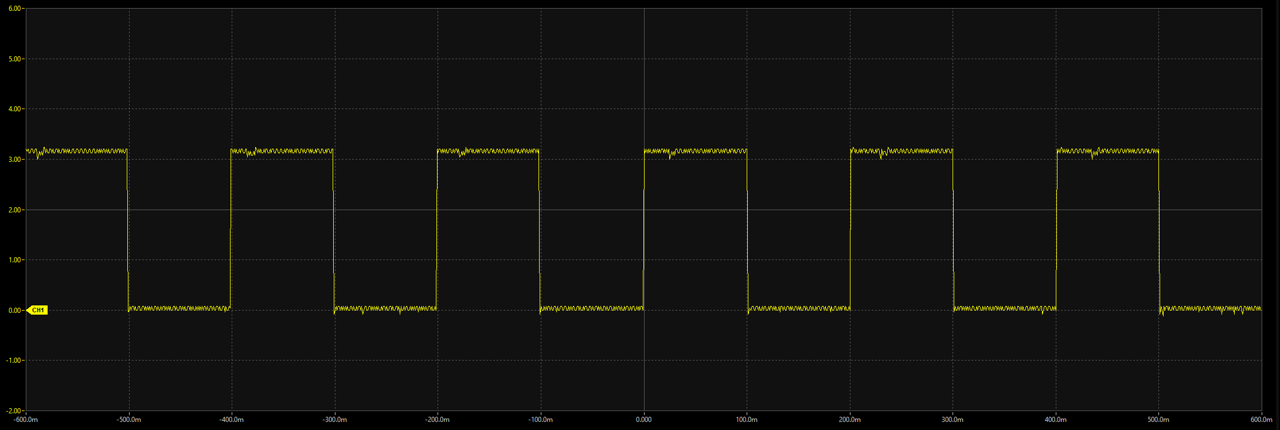
\includegraphics[width=1\columnwidth]{chapters/development/results/DELAY}
\end{figure}

With the system clock frequency set correctly, debugging works on the device and the CPU can be halted and stepped through instructions as the program is running.

\subsection{ESP32 Control}
The ESP32 is controlled by the PIC32 in two ways.

\begin{itemize}
        \item The ESP32 enable pin is connected to pin 14 (RB2) of the PIC32.
        \item The ESP32 HSPI bus is connected to SPI2 of the PIC32
\end{itemize}

The enable pin of the ESP32 just needs to be asserted high, which can be done by the PIC32 using the code shown in~\autoref{code:esp_en}

\begin{lstlisting}[language=C,caption={PIC32 code for enabling the ESP32}\label{code:esp_en}]
  void ESP32_IO_init() {
    TRISBbits.TRISB2 = 0;       // Set ESP32 EN pin as output
    PORTBbits.RB2 = 1;          // Set ESP32 EN pin high
  }
\end{lstlisting}

Without this assertion, the ESP32 is unresponsive to programming and does not perform code execution.

The other form of control is through the respective SPI lines of the two microcontrollers.
The SPI driver for the PIC32 is simple, as that device acts as the `master', which is the typical mode for a microcontroller to operate in.
The PIC32 is configured as a 32-bit master operating in SPI mode 3~\cite{Barry:2012}.
The baudrate generator value has been calculated using the equation \(BRG = (F_{PB} / 2 \times F_{SCK}) - 1\),
and a SPI clock speed of 31.3 kHz has been generated (using a BRG value of 50).
This value has been intentionally set low so that the transmission speeds are well below what both devices are capable of,
they can be easily raised by decreasing the value of BRG, once the system has been well tested.
Finally, the low-level SPI driver is implemented in~\autoref{code:spi_driver}

\begin{lstlisting}[language=C,caption={PIC32 low-level SPI driver}\label{code:spi_driver}]
  uint32_t ESP32_SPI_write(uint32_t data) {
    SPI2BUF = data;
    while(!SPI2STATbits.SPITBE);
    uint32_t read = SPI2BUF;

    delay_us(5000);
    return read;
  }
\end{lstlisting}

The function of the code is relatively straightforward.
The memory location of the SPI2BUF variable is mapped to the SPI 2 peripheral.
When written to, the data at this address is written into a transmit buffer that queues the data for SPI transmission.
When read from, data that has been received by the SPI peripheral is taken from the receive buffer.
Between these two operations the processor waits for the SPITBE status flag to be set.
This flag corresponds to the transmission buffer being empty, and is set once transmission has been completed and data has been received.

Additionally, a delay is required between SPI writes in order to stop data from becoming corrupt.
This delay was embedded into the low-level driver to make eventual performance optimization centralized,
since this delay is a clear cost to performance and by far the cause of the most communication slowdown.
This delay is most likely necessary due to the operation of the SPI chip select line.
Specifically, the way the chip select line does not reset between SPI transmissions without adequate delays between writes.
This could be solved by manually asserting the chip select line instead of allowing the peripheral to control it.
However, due to time restrictions it was decided that features should be implemented in a basic functional form,
and performance could be optimized once the system was fully functional.
and thus the driver was implemented using significantly slower delay.

The ESP32 SPI configuration was less straightforward.
As microcontrollers are typically the devices that coordinate communication between various `dumb' sensors,
they almost always act as the SPI master.
However, since the on-body device uses multiple microcontrollers communicating via SPI,
one of these devices needs to act as a slave.
Since the PIC32 is what communicates to the sensors, and the ESP32 only acts as a wireless transmitter,
the PIC32 was configured as the SPI master, leaving the ESP32 as an SPI slave.
There no official support for this in the native development environment, so a third party library was used.

The library that was used is the ESP32DMASPI library~\cite{ESP32DMASPI}.
This library is based on the official driver from the manufacture~\cite{SPI}.

SPI was implemented using task based DMA receiving.
In this setup, tasks run in separate threads, which frees up main thread to only process OTA updates.
One task runs continuously, waiting for SPI transmission~\autoref{code:esp_spi}.
% TODO: DESCRIBE IN MORE DETAIL HOW THESE WORK
%
\begin{lstlisting}[language=C++,caption={ESP32 code for receiving SPI data}\label{code:esp_spi}]
  void task_wait_spi(void* pvParameters) {
    while (1) {
      ulTaskNotifyTake(pdTRUE, portMAX_DELAY);
      slave.wait(buffer, BUFFER_LENGTH);
      xTaskNotifyGive(task_handle_process_buffer);
    }
  }
\end{lstlisting}

Once data has been received, a different task handles processing the incoming data~\autoref{code:esp_spi_processing}.

\begin{lstlisting}[language=C++,caption={ESP32 code for processing SPI data}\label{code:esp_spi_processing}]
  void task_process_buffer(void* pvParameters) {
    while (1) {
      ulTaskNotifyTake(pdTRUE, portMAX_DELAY);
      print_array(buffer, slave.available());
      slave.pop();
      xTaskNotifyGive(task_handle_wait_spi);
    }
  }
\end{lstlisting}

This should have been the end of the SPI implementation,
however the SPI communication did not work with just this code.
To get the communication working some additional functions were required on the PIC.
For example, the only way to send data was to write a single byte at a time, despite the fact that the SPI module is in 32-bit (4 byte) mode.
What is interesting about this is that the single byte must be located at the front of the 4 byte word.
This implies that the ESP32 was not able to receive 32-bits, and instead was just receiving the first 8-bit word.
However, if the SPI peripheral of the PIC32 was put into 8-bit mode (and all respective code changed to fit that mode),
the ESP32 would receive nothing.
So, the ESP32 required the PIC32 to send 32 SPI clock pulses but would only receive the first 8 data bits.
This same behavior was present when using both a task based approach or a polling approach and when DMA was or was not in use.
It is a substantial issue because it adds a 75\% overhead to the communication system.
This, and the required delay in the low-level driver, are the primary candidates for future optimizations.
The code for embedding data into a 4 byte word is shown in~\autoref{code:spi_additional_functions}.

\begin{lstlisting}[language=C++, caption={PIC32 additional SPI functions}\label{code:spi_additional_functions}]
  void ESP32_SPI_write_4byte(uint8_t b1, uint8_t b2, uint8_t b3, uint8_t b4) {
    uint32_t word = ((uint32_t)b1 << 24)
                  | ((uint32_t)b2 << 16)
                  | ((uint32_t)b3 << 8)
                  | (uint32_t)b4;

    ESP32_SPI_write(word);
  }

  void ESP32_SPI_write_byte(uint8_t data) {
    ESP32_SPI_write_4byte(data, 0, 0, 0);
  }
\end{lstlisting}

Despite significant performance issues, the drivers function together.
Allowing abritary bytes to be shared between the two devices.


\section{ADS1294R}
The ADS1294R is a 4 channel, 24-bit, delta-sigma analog-to-digital converter with additional features to support electrocardiogram and electroencephalogram measurements.
This device is the primary sensor front end.
It communicates with the PIC32 via SPI as well as several hardware control lines.

\subsection{Design Differences}
Like the PIC32, the schematic for the ADS1294R were slightly different to what was assembled due to chip shortages.
The schematic showed the devices as an ADS1298R, which is the 8 channel version of the device.
This is significant because the device requires a specific number of SPI clock pulses to be sent that correlates to the number of channels on the device.
So sending the wrong number of clock pulses will generate undesired results.
Additionally, the device ID is different which can cause some confusion when initially trying to configure the device.

\subsection{Startup Procedure}
The startup procedure of the device is shown in~\autoref{fig:ads_startup}.
When implementing this startup procedure, a similar SPI driver to what was seen in~\autoref{code:spi_driver} was used.
The key difference is that a higher delay was used for testing to ensure communication was well below data sheet limitations~\cite{ADS}.
When trying to follow this procedure, there were a number of key differences between what was expected and what was measured.
It appeared that no matter what command was sent, the response was always the binary number \(01100000\).
The data sheet specified responses for different registers, but regardless of the register the response was always the same.
The device also did not appear to respond to any two byte commands.
However, the device did respond to single byte commands.

\begin{figure}[!ht]
  \caption{ADS1294R startup sequence}\label{fig:ads_startup}
  \centering
  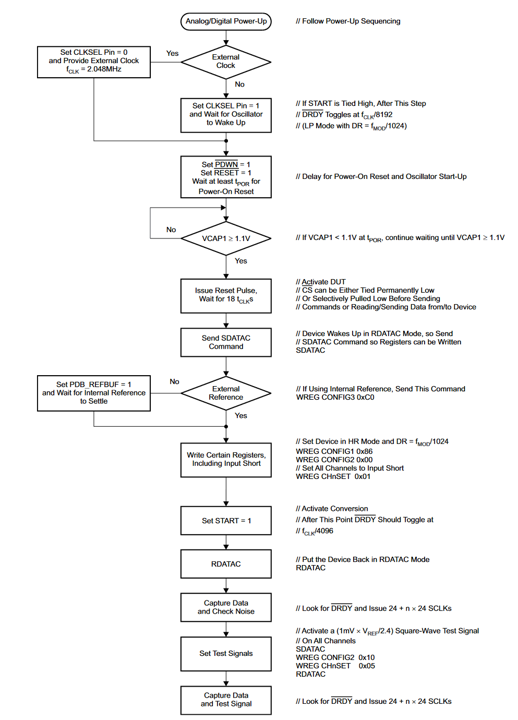
\includegraphics[width=1\columnwidth/2]{chapters/development/results/ADS_Startup_Sequence}
\end{figure}

The single byte commands were verified by monitoring the state of the data ready pin.
Since this pin was connected to the PIC and the PIC has general purpose test points on a number of pins;
the read value of the data ready pin can be written to one of the test points.
This effectively `passes through' the state of the pin.
The caveat being that any delays to the PIC will cause a delay between the data ready value and the test point.
As well as that it strips the signal of all information aside from if it has crossed the PIC's logic threshold.
However, the limited information it provides is still useful in this context.
Using an oscilloscope connected to the `pass through' test point, it is shown that the data ready pin is continually asserted.
This changes after calling single byte commands that change the state of the ADS1294R.
For example, if the reset command is continually send, the data ready pin will never be asserted,
once the command stops being sent, the data ready pin is reasserted.
Similarly, if the standby or stop commands are sent, the pin is not asserted until the respective wakeup or start commands are sent.
The exact same behavior is observed when the physical reset pin is held down, or when the start pin is asserted by the PIC.
What this says is that the device is powered and the transmit side of the SPI bus is connected correctly.
Since the SPI binary response is always \(01100000\), it can be assumed that the receive side of the SPI bus is also connected correctly.
This is because the response does not change and is both non-zero and also not continually driven high.
If either of those were true, the SPI bus could be picking up noise, or the receive pin may not be getting asserted.
But because of this response it must be being controlled by the ADS1294R SPI module,
since there is no other part of that device that is connected to the SPI clock and the response is the same even at higher and lower SPI clock speeds.

As the SPI hardware is assumed to be connected correctly, and the low-level SPI driver is confirmed to work with the ESP32,
the fault is assumed to be in the SPI configuration and startup procedure on the PIC.
Changing the clock polarity or clock phase causes the single byte commands to fail.
On top of that, changing the SPI interface off of 8-bit mode to 32-bit or 16-bit mode also caused the commands to fail.
The only change that could be made was the data sampling time, as this effected nothing to do with the transmission.
This change caused the received bits to change position,
but they were still not correct and different commands still caused the device to respond with the same response each time.
Therefore, the place in the program that was most widely explored was the code for the startup procedure.

The most obvious difference is that the startup procedure suggests using the hardware reset,
but that pin is tied to a physical switch instead of directly connected to the PIC.
Because of this, there is no way to automatically hardware reset the device in software,
so the reset has previously been achieved by sending the reset command.
To achieve a true hardware reset, a long delay was added to the startup sequence so that the physical switch could be pressed with the correct timing.
To aid with the timing, one of the test points was also driven high at the start of this timing window and low once the window had passed.
Then, using an oscilloscope to verify the timing window, the ADS1294R could be hardware reset at the correct point in the boot-up process.
This unfortunately did not solve the issue and the device still maintained the same issue as before.

Next, the register read and register write functions were investigated.
Since we had verified that the low-level driver was functional, and that same driver handled both the reading and writing,
it was unlikely that this was the issue, as this driver is so simple ther are not many places errors could propagate.

The code for writing to the register is shown in~\autoref{code:ads_reg_write}.

\begin{lstlisting}[language=C, caption={PIC32 code for writing ADS1294R register}\label{code:ads_reg_write}]
  void write_register(uint8_t reg, uint8_t data) {
    static uint8_t write_register_cmd = 0x40;
    static uint8_t write_register_mask = 0x1F;

    uint8_t first_byte = write_register_cmd | (reg & write_register_mask);
    uint8_t second_byte = 0x00; // only ever write a single register

    ADS1294R_write(first_byte);
    ADS1294R_write(second_byte);
    ADS1294R_write(data);
  }
\end{lstlisting}

As the write commands were verified to be working, the changes to this function were around the register command byte,
register mask byte, and the addition of delays between writing the bytes.
However, these changes did not have any effect on the communication issues with the device.
We then turned our attention to the read register function shown in~\autoref{code:ads_reg_read}

\begin{lstlisting}[language=C, caption={PIC32 code for reading ADS1294R register}\label{code:ads_reg_read}]
  uint8_t read_register(uint8_t reg) {
    static uint8_t read_register_cmd = 0x20;
    static uint8_t read_register_mask = 0x1F;

    uint8_t first_byte = read_register_cmd | (reg & read_register_mask);
    uint8_t second_byte = 0x00; // only ever read a single register

    ADS1294R_write(first_byte);
    ADS1294R_write(second_byte);
    return ADS1294R_read();
  }
\end{lstlisting}

Similar changes and additions were added to this function, with the same result of the communication not working correctly.

At this point all of the command and register definition were double checked and
the register read and write functions were stepped through to verify that the bytes bit by bit, and all confirmed to be correct.

Since all logical software changes had been made and the system was still not functional,
it was decided that the SPI pins should be broken out so the commuincation could be analyzed using an oscilloscope.
Craig Dawson from engineering services helped in this aspect of the project,
since the pitch of the pins that needed to be soldered required specialized tools and expertise.
The device modifications are shown in~\autoref{fig:pic_wires}.

\begin{figure}[!ht]
  \caption{PIC32 board attached debugging wires}\label{fig:pic_wires}
  \centering
  \includegraphics[width=1\columnwidth]{chapters/development/results/P_20230919_170532}
\end{figure}


A four channel oscilloscope could then be used to analyze the SPI communication.
What was eventually discovered was that the chip select pin was not being asserted for long enough.
The SPI communication between the two devices is shown in~\autoref{fig:ads_spi}.
Since the chip select pin was being controlled by the PIC SPI module,
it was being automatically driven low during transmission and then high again after transmission completed.
This would have been the desired behavior, and it indeed was for single byte commands,
but for multi-byte commands the chip select line needed to stay asserted until all of the bytes had been transferred and received.

\begin{figure}[!ht]
  \caption{SPI communication between PIC32 and ADS1294R}\label{fig:ads_spi}
  \centering
  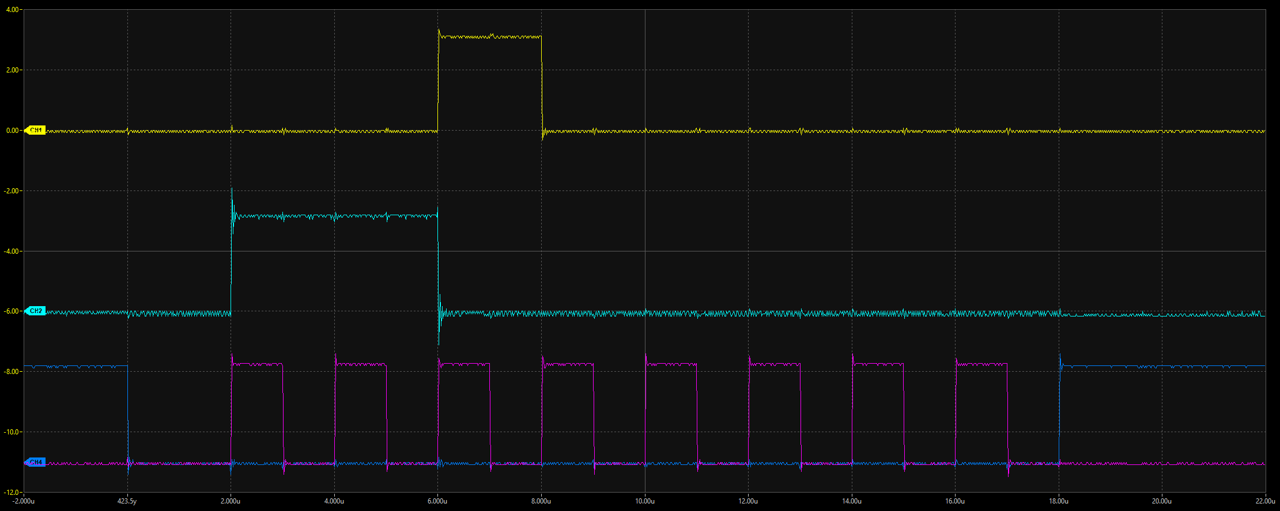
\includegraphics[width=1\columnwidth]{chapters/development/results/ADS_SPI_COMMS}
\end{figure}

The solution to this is to disable chip select control on the SPI module and manually set and reset the pin in software.
To accomplish this, the code was changed as shown in~\autoref{code:ads_cmd_write} and~\autoref{code:ads_updated_reg_funcs}

\begin{lstlisting}[language=C, caption={PIC32 code for writing single-byte commands to the ADS1294R}\label{code:ads_cmd_write}]
  void write_cmd(uint8_t cmd) {
    CS_PIN = 0;   // Chip select pin is active low
    ADS1294R_write(cmd);
    CS_PIN = 1;   // Chip select pin in inactive high
  }
\end{lstlisting}


\begin{lstlisting}[language=C, caption={PIC32 code for writing single-byte commands to the ADS1294R}\label{code:ads_updated_reg_funcs}]
  uint8_t read_register(uint8_t reg) {
    static uint8_t read_register_cmd = 0x20;
    static uint8_t read_register_mask = 0x1F;

    uint8_t first_byte = read_register_cmd | (reg & read_register_mask);
    uint8_t second_byte = 0x00; // only ever read a single register

    CS_PIN = 0;
    ADS1294R_write(first_byte);
    ADS1294R_write(second_byte);
    ADS1294R_read();
    uint8_t ret = ADS1294R_read();
    CS_PIN = 1;

    return ret;
  }

  void write_register(uint8_t reg, uint8_t data) {
    static uint8_t write_register_cmd = 0x40;
    static uint8_t write_register_mask = 0x1F;

    uint8_t first_byte = write_register_cmd | (reg & write_register_mask);
    uint8_t second_byte = 0x00; // only ever write a single register

    CS_PIN = 0;
    ADS1294R_write(first_byte);
    ADS1294R_write(second_byte);
    ADS1294R_write(data);
    CS_PIN = 1;
  }
\end{lstlisting}

With these changes, communication with the device is established and the device ID can be read successfully.

\chapter{Integration}
ESP32 Wireless Comms -> Plotting Data Wirelessly -> PIC32 SPI Comms -> PIC32 Wireless Comms -> Printf WiFi Debugging -> ADS1294R SPI Comms -> Power Issues

\section{Off-Body PC}
This device must receive data wirelessly from the on-body device and processes it for music and lighting generation.

\lstinputlisting[language=MATLAB]{chapters/development/MATLAB/TCPIP_EXAMPLE.m}
\lstinputlisting[language=MATLAB]{chapters/development/MATLAB/TCPIP.m}

\subsection{Wireless Transmission}

Before I was filling a buffer from the incoming data and waiting until I received
a newline before sending the entire buffer over TCP/IP all at once.
Now I receive data and immediately send, provided client.connected()
I use slave.available() to specify the length of data to be sent.

This is better because it keeps the TCP/IP transmitter simple and also allows all
of the packet metadata to be changeable independently of the ESP.

Currently having a number of IO issues with the PIC32.
Seems like no matter how I set the IO register direction, or how I set
the PORT or LATCH bits, the IO pin never changes.
I appear to be able to correctly read from the IO port although this
hasn't been fully tested I am just able to see ports that should be
inputs driven high.

It may be worth setting those to outputs and see if I still read them
as inputs because it seems like there is no pin assertion happening.

Setting the TRIS bit and then writing the PORTx bit high is all that
needs to be done.
I can verify this because the ESP32 needs its enable pin to be pulled
high and that is done sucesfully using `TRISBbits.TRISB2 = 0;' and
`PORTBbits.RB2 = 1;'
(testing this by setting `PORTBbits.RB2 = 0' resulted in the ESP
shutting down)
It just seems that no matter what I do, I cannot get signal on any of
the test points. I'm trying to determine if it's an issue with the
program or if the pinout is incorrect or if the routing was not done
properly or some other issue like maybe my scope isn't referenced to
the correct ground and the voltage that is present is actually not
being measured.

I'm thinking a reasonable way to proceed would be to continuity test
a specific pin and 100\% verify the port and pin before checking it just
with the multimeter to determine if voltage is present. Then, once that
has be sorted move on to using the scope.
What do we know:

    - Pin outputs are set using TRISx and PORTx.
    - The enable pin for the ESP is using one of these pins
        - Although all that I've really been seeing
        is the brownout detector being triggered
        so maybe the ESP not working is unrelated to the
        tampering I was doing with that pin...
    - I am not able to see changes on any of the test points
        - This is really strange because I am setting the entire port
        worth of pins so I don't see how they could be getting missed.

I think it's worth investigating the ESP enable pin a little closer.
Maybe check voltage with a multimeter since it should be pretty easy.
Then, if there is voltage attempt to remove and see what the ESP does
(when properly powered using external supply as to not trip
brownout detection).
Then continue to different pin on same port, verify that is also working.
Finally, attempt changing port and test off pin of controller.
Continuity test between pin and test point then check test point.
If all correct we know 100% that the issue is with the scope.

Might have something to do with the brownout detector that the ESP is constantly triggering.
Think this is because the board requires more power to perform specific actions.
For instance, I think the PIC debugging requires a bit of power because of the speed,
and when it happens the ESP voltage drops low enough that it causes a brownout.
My solution to this is to decrease the clock speed of the PIC since the 80MHz is much
faster than what we actually need the system to ever run at considering the requirements.

Slowing the clock speed did not fully solve the issue and sometime the brownout detector
is tripped again...
Attempting to solve by plugging in a short USB into port of board.
Also need to enable ICD 3 powering of board.

\section{System Integration}
With the on-body device as a single block, how the system has been fully integrated.

\subsection{Packet Based Approach}
Sending bytes between the devices work

%\lstinputlistinglanguage=C{chapters/research/package_test/simple.c}
The packet is made up of a struct containing bit length defs
for each of data types we will be sending.

This struct is then treated as an array and encoded using base64
(decision matrix pending).

The encoded data is then sent via SPI to the ESP32 which acts
as a SPI slave that simply receives any amount of data
(less than 1024 bytes long) and transmits it once it receives
the end of line character (`\\n').
This character is hard coded but it also required to be present
for the MATLAB code to function so it is consistent across both.

The challenge now is that the data needs to be decoded in MATLAB.
The following code can be used in a callback function to convert
the received encoded data into an array of byte values.

\begin{lstlisting}[language=MATLAB]
base64 = readline(src);
decoded = transpose(matlab.net.base64decode(char(base64)));
\end{lstlisting}

The decoded data can then be converted into the correct format
using the following code

\begin{lstlisting}[language=MATLAB]
x = uint8(decoded(9:12));
disp(typecast(x, 'uint32'))
\end{lstlisting}

The issue here is that there is a lot of hardcoded values
in both the index of the data and the conversion format.
One solution is to remove all bit length defs and send everything
as 32-bit words. The tradeoff is that it is potentially quite wasteful.
For instance, if we only needed to send 8-bits, we are essentially
sending 24-bits of unnecessary data that will all be 0s.

We ideally want to send a header at the start of transmission that
contains all the information regarding size of data, etc.
Then send a packet identifier so the system knows what data to expect.

What would be good is to have all the identifiers be bitwise OR'd
with each other so that the MATLAB code can just look at the identifier
bit and can tell which pieces of data are present.
This is better than the alternative of having seperate identifiers for
every combination of data because then we can just define everything once.
For example our header could look like the following:

\begin{lstlisting}[language=C]
IDENTIFIER = 0b10011000
\end{lstlisting}

which might correspond to ECG data, RESP data, and EMG data.
The definitions for those data masks could be as follows:

\begin{lstlisting}[language=C]
ECG_MASK = 0b10000000
RSP_MASK = 0b00010000
EMG_MASK = 0b00001000
\end{lstlisting}

We could see from this that the identifier contains the corresponding
masks and use it to extract the data.
We could then say that the highest mask takes prescience.
So, in this example the ECG data would come first since its mask's bit
is the highest in the identifier.

Then, all we need to define is that the mask bit corresponds to x amount
of data. So that once we see a specific mask bit is set we can
automatically align the data.

I think its best to do this first manually by having all the masks
and sizes set. Then, once that is working move to having a config packet
that sets the masks and sizes dynamically.
The goal is to keep the definitions in once place and propagate it
through the system.

Wrote a debug routine to print arbritary text to MATLAB via SPI/TCP.

\begin{lstlisting}[language=C]
void debug(const char *fmt, ...) {
    va_list args;
    char str[1024];

    va_start(args, fmt);
    vsprintf(str, fmt, args);
    va_end(args);

    write_packet(str, strlen(str));
}
\end{lstlisting}

Then can receive in MATLAB using

\begin{lstlisting}[language=MATLAB]
y = char(decoded);
disp(y)
\end{lstlisting}


\section{Testing and Validation}
What tests were performed and how that validates the system.

\chapter{Future Work}
What can be done going forward

\chapter{Conclusion}
This project was a continuation of the Music from Biosignals project.
It focussed on developing the hardware for biosignal acquisition, and a controller for controlling lighting fixtures.
The project was successful in creating the lighting controller, as well as programming the hardware.
However, due to previous board design issues, the devices were not able to be powered together.
Therefore, while the device to device connections on the board were tested and working,
the fully system integration was not able to be completed.

This project succeeded in demonstrating the design flaws of the on-body device, while also providing a number of recommendations for a future redesign.


%----------------------------------------------------------------------------------------
%	BIBLIOGRAPHY
%----------------------------------------------------------------------------------------

\printbibliography{}

%---------------------------------------------------------------------------------------
%	THESIS CONTENT - APPENDICES
%----------------------------------------------------------------------------------------

\appendix % Cue to tell LaTeX that the following "chapters" are Appendices

% Include the appendices of the thesis as separate files from the Appendices folder
% Uncomment the lines as you write the Appendices

% TODO: eventually need to get this working
% for some reason makefile does not allow access to this directory

\chapter{Gantt Chart}\label{appendix:gantt}

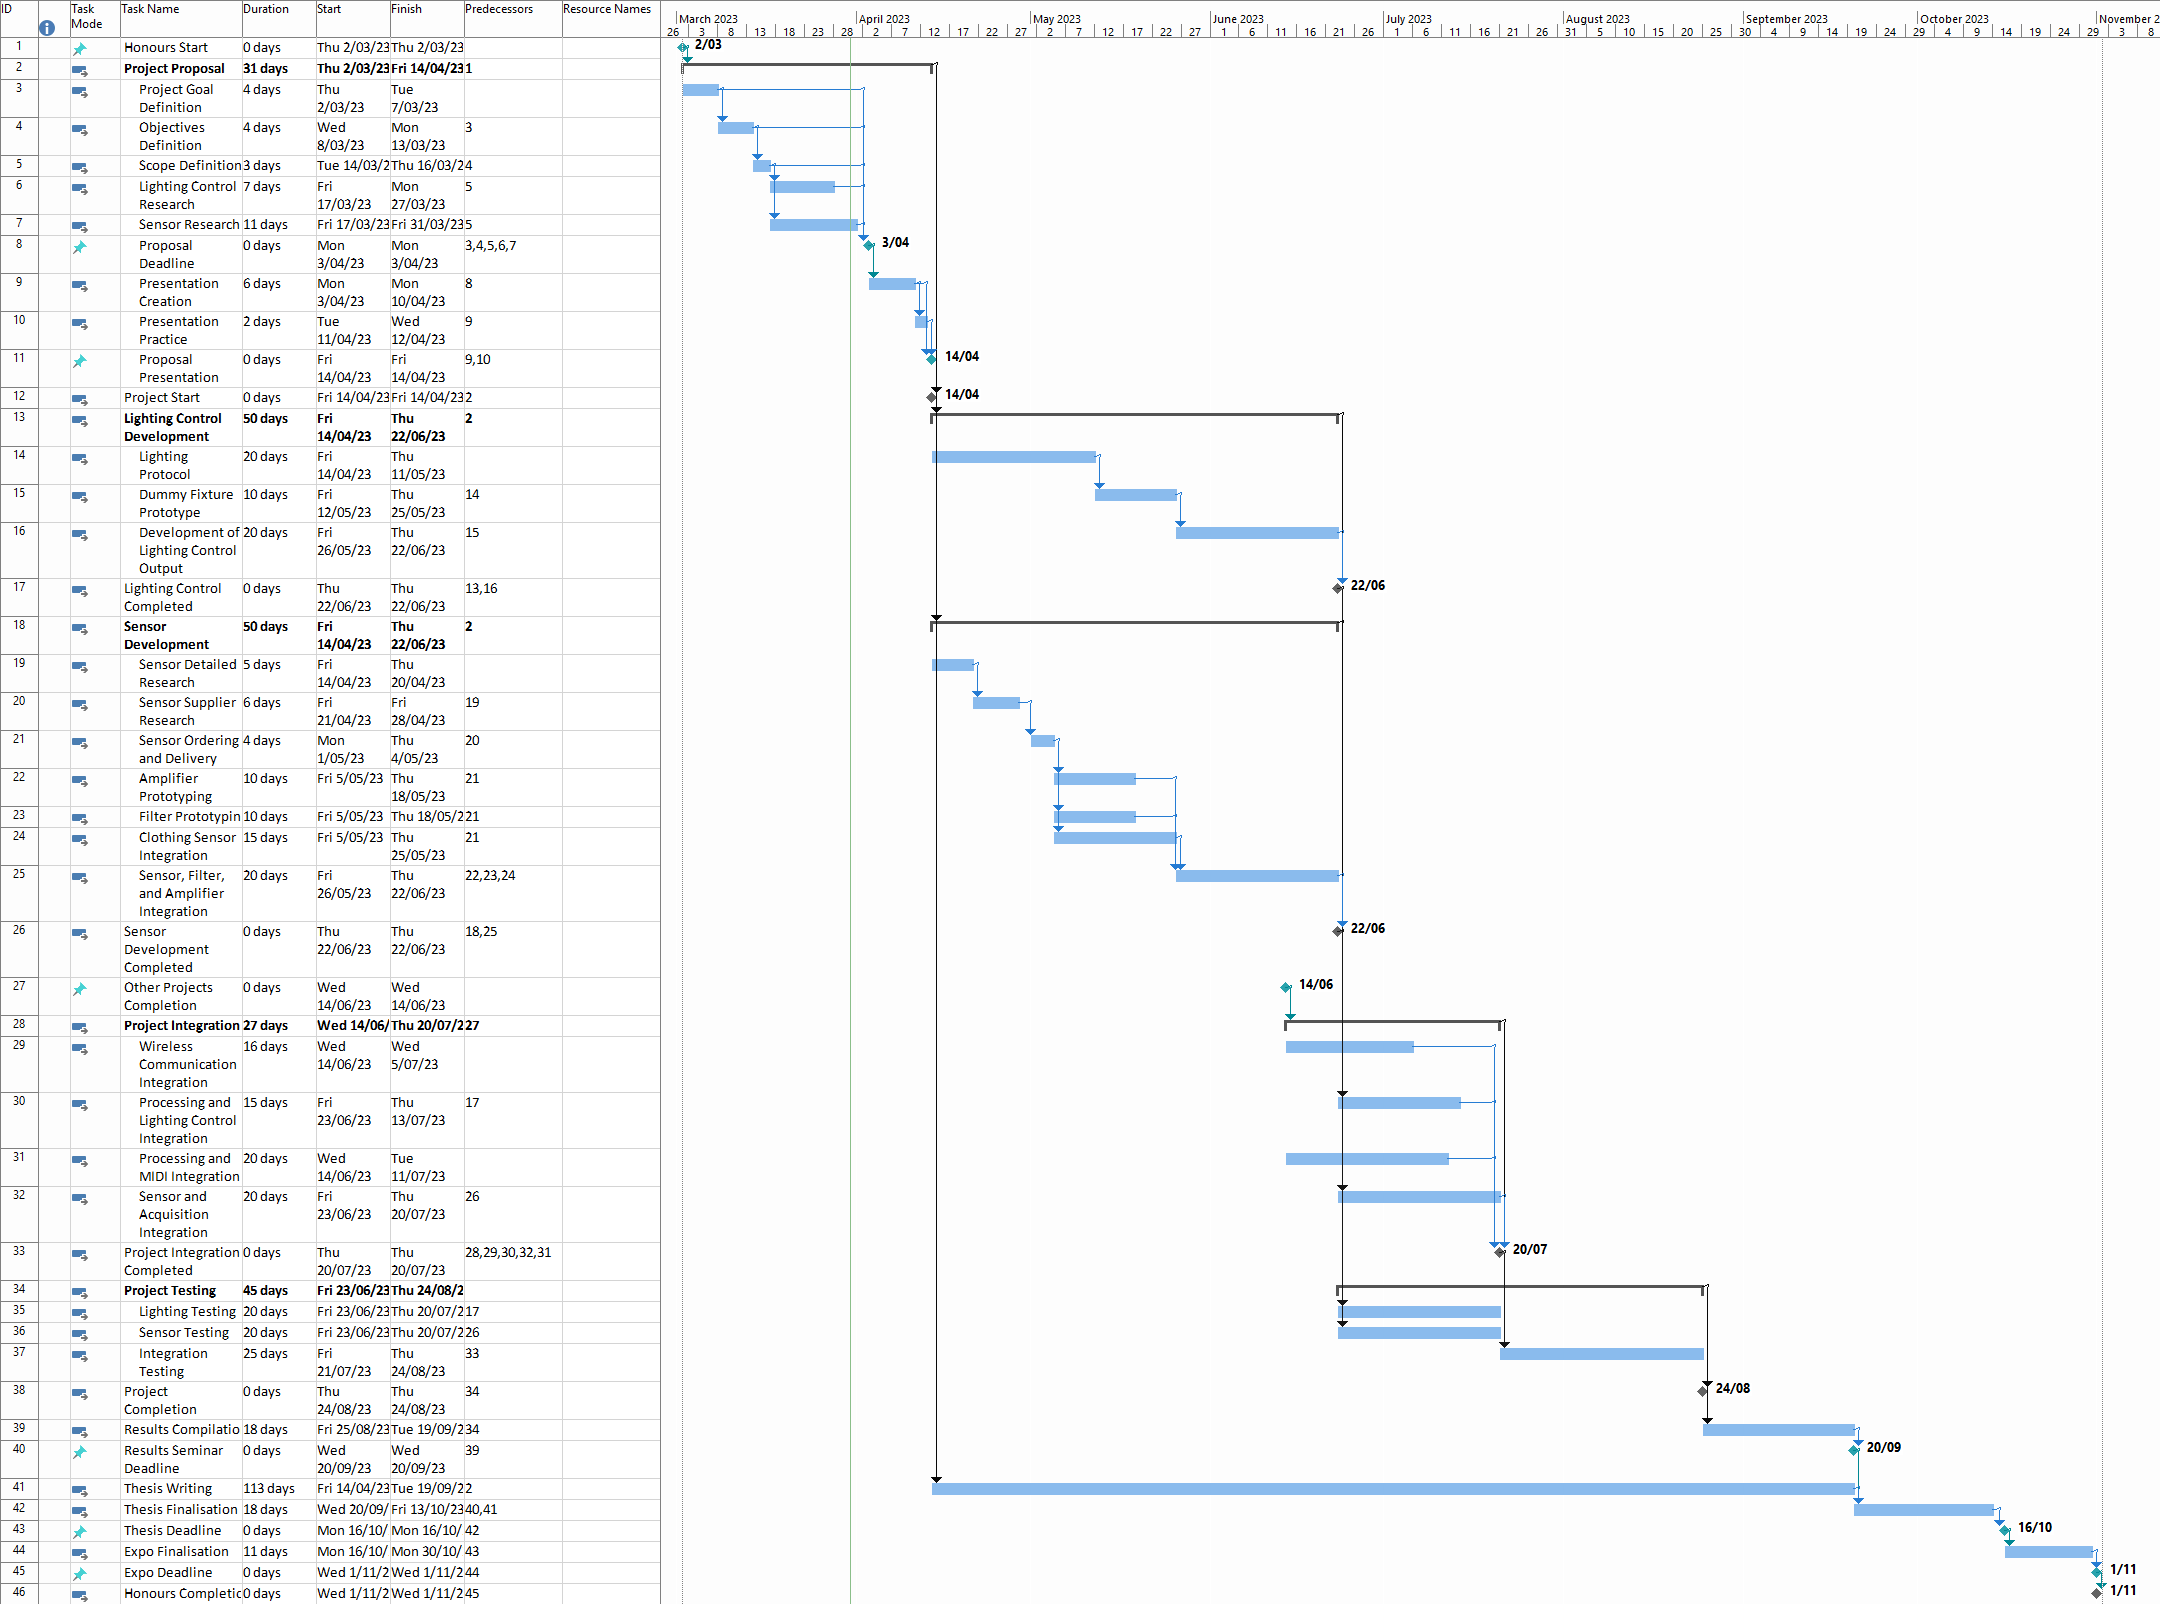
\includegraphics[width=1\columnwidth]{chapters/project_plan/figures/Gantt_Chart}

\chapter{Prototyping Fixture Code}\label{appendix:prototyping_fixture}

\begin{lstlisting}[language=C++]
#include <stdint.h>
#include <stdio.h>
#include <string.h>
#include <Adafruit_NeoPixel.h>
#include <Base64.h>

#define PIXELS_PIN 6
#define NUM_PIXELS 8
#define ADDR_PER_PIXEL 4
#define DMX_LENGTH (NUM_PIXELS * ADDR_PER_PIXEL)
#define UNIVERSE_SIZE 32

#define INPUT_BUFFER_LENGTH 1024
#define BASE64_LENGTH 128
#define RAW_LENGTH 95

Adafruit_NeoPixel pixels(NUM_PIXELS, PIXELS_PIN, NEO_GRB + NEO_KHZ800);
uint8_t dmx_values[UNIVERSE_SIZE];

char input_buffer[INPUT_BUFFER_LENGTH];
char decode_buffer[BASE64_LENGTH];
uint16_t input_index = 0;
uint8_t new_data = 0;

void setup() {
  Serial.begin(115200);
  pixels.begin();
  pixels.clear();
  pixels.show();
}

void serialEvent() {
  while (Serial.available()) {
    if (input_index > INPUT_BUFFER_LENGTH) { input_index = 0; } // Should never hit this
    char c = Serial.read();

    if (c == '\n') {
      memset(decode_buffer, '\0', BASE64_LENGTH);
      memcpy(decode_buffer, input_buffer, input_index);
      new_data = 1;
      input_index = 0;
      continue;
    }

    input_buffer[input_index++] = c;
  }
}

void loop() {
  if (new_data) {
    new_data = 0;

    int decoded_length = Base64.decodedLength(decode_buffer, BASE64_LENGTH);
    char decoded_string[decoded_length];
    Base64.decode(decoded_string, decode_buffer, BASE64_LENGTH);

    int array_index = 0;
    for (int i = 0; i < decoded_length; i += 3) {
      char val[3];
      val[0] = (decoded_string[i+0]);
      val[1] = (decoded_string[i+1]);
      val[2] = (decoded_string[i+2]);

      dmx_values[array_index++] = atoi(val);
    }

    for (int addr = 0; addr < DMX_LENGTH; addr += ADDR_PER_PIXEL) {
      uint8_t i = dmx_values[addr + 0];
      uint8_t r = dmx_values[addr + 1];
      uint8_t g = dmx_values[addr + 2];
      uint8_t b = dmx_values[addr + 3];

      uint32_t color = pixels.Color(
        (r * i) >> 8,
        (g * i) >> 8,
        (b * i) >> 8
      );

      pixels.setPixelColor(addr / ADDR_PER_PIXEL, color);
    }

    pixels.show();

  }
}

\end{lstlisting}

\chapter{DMX Server Code}\label{appendix:dmx_server}

\begin{lstlisting}[language=C++]
using System;
using System.Runtime.InteropServices;
using System.IO;
using System.Threading;

namespace DMXServer
{

    public class OpenDMX

    {

        public static byte[] buffer = new byte[513];
        public static uint handle;
        public static bool done = false;
        public static int bytesWritten = 0;
        public static FT_STATUS status;
        public static Thread thread;

        public const byte BITS_8 = 8;
        public const byte STOP_BITS_2 = 2;
        public const byte PARITY_NONE = 0;
        public const UInt16 FLOW_NONE = 0;
        public const byte PURGE_RX = 1;
        public const byte PURGE_TX = 2;



        [DllImport("FTD2XX.dll")]
        public static extern FT_STATUS FT_Open(UInt32 uiPort, ref uint ftHandle);
        [DllImport("FTD2XX.dll")]
        public static extern FT_STATUS FT_Close(uint ftHandle);
        [DllImport("FTD2XX.dll")]
        public static extern FT_STATUS FT_Read(uint ftHandle, IntPtr lpBuffer, UInt32 dwBytesToRead, ref UInt32 lpdwBytesReturned);
        [DllImport("FTD2XX.dll")]
        public static extern FT_STATUS FT_Write(uint ftHandle, IntPtr lpBuffer, UInt32 dwBytesToRead, ref UInt32 lpdwBytesWritten);
        [DllImport("FTD2XX.dll")]
        public static extern FT_STATUS FT_SetDataCharacteristics(uint ftHandle, byte uWordLength, byte uStopBits, byte uParity);
        [DllImport("FTD2XX.dll")]
        public static extern FT_STATUS FT_SetFlowControl(uint ftHandle, char usFlowControl, byte uXon, byte uXoff);
        [DllImport("FTD2XX.dll")]
        public static extern FT_STATUS FT_GetModemStatus(uint ftHandle, ref UInt32 lpdwModemStatus);
        [DllImport("FTD2XX.dll")]
        public static extern FT_STATUS FT_Purge(uint ftHandle, UInt32 dwMask);
        [DllImport("FTD2XX.dll")]
        public static extern FT_STATUS FT_ClrRts(uint ftHandle);
        [DllImport("FTD2XX.dll")]
        public static extern FT_STATUS FT_SetBreakOn(uint ftHandle);
        [DllImport("FTD2XX.dll")]
        public static extern FT_STATUS FT_SetBreakOff(uint ftHandle);
        [DllImport("FTD2XX.dll")]
        public static extern FT_STATUS FT_GetStatus(uint ftHandle, ref UInt32 lpdwAmountInRxQueue, ref UInt32 lpdwAmountInTxQueue, ref UInt32 lpdwEventStatus);
        [DllImport("FTD2XX.dll")]
        public static extern FT_STATUS FT_ResetDevice(uint ftHandle);
        [DllImport("FTD2XX.dll")]
        public static extern FT_STATUS FT_SetDivisor(uint ftHandle, char usDivisor);


        public static void start()
        {
            handle = 0;
            status = FT_Open(0, ref handle);
            thread = new Thread(new ThreadStart(writeData));
            thread.Start();
            setDmxValue(0, 0);  //Set DMX Start Code
        }

        public static void stop()
        {
            if (thread != null && thread.ThreadState != ThreadState.Stopped)
            {
                thread.Abort();
            }

            status = FT_Close(handle);
        }

        public static void setDmxValue(int channel, byte value)
        {
            if (buffer != null)
            {
                buffer[channel + 1] = value;
            }
        }

        public static void writeData()
        {
            while (!done)
            {
                initOpenDMX();
                FT_SetBreakOn(handle);
                FT_SetBreakOff(handle);
                bytesWritten = write(handle, buffer, buffer.Length);
                Thread.Sleep(20);
            }

        }

        public static int write(uint handle, byte[] data, int length)
        {
            IntPtr ptr = Marshal.AllocHGlobal((int)length);
            Marshal.Copy(data, 0, ptr, (int)length);
            uint bytesWritten = 0;
            status = FT_Write(handle, ptr, (uint)length, ref bytesWritten);
            return (int)bytesWritten;
        }

        public static void initOpenDMX()
        {
            status = FT_ResetDevice(handle);
            status = FT_SetDivisor(handle, (char)12);  // set baud rate
            status = FT_SetDataCharacteristics(handle, BITS_8, STOP_BITS_2, PARITY_NONE);
            status = FT_SetFlowControl(handle, (char)FLOW_NONE, 0, 0);
            status = FT_ClrRts(handle);
            status = FT_Purge(handle, PURGE_TX);
            status = FT_Purge(handle, PURGE_RX);
        }

    }

    /// <summary>
    /// Enumaration containing the varios return status for the DLL functions.
    /// </summary>
    public enum FT_STATUS
    {
        FT_OK = 0,
        FT_INVALID_HANDLE,
        FT_DEVICE_NOT_FOUND,
        FT_DEVICE_NOT_OPENED,
        FT_IO_ERROR,
        FT_INSUFFICIENT_RESOURCES,
        FT_INVALID_PARAMETER,
        FT_INVALID_BAUD_RATE,
        FT_DEVICE_NOT_OPENED_FOR_ERASE,
        FT_DEVICE_NOT_OPENED_FOR_WRITE,
        FT_FAILED_TO_WRITE_DEVICE,
        FT_EEPROM_READ_FAILED,
        FT_EEPROM_WRITE_FAILED,
        FT_EEPROM_ERASE_FAILED,
        FT_EEPROM_NOT_PRESENT,
        FT_EEPROM_NOT_PROGRAMMED,
        FT_INVALID_ARGS,
        FT_OTHER_ERROR
    };

}

\end{lstlisting}

\begin{lstlisting}[language=C++]
using System;
using System.Threading;
using System.IO.Ports;
using System.Linq;

namespace DMXServer
{
    public class ArduinoDMX
    {
        static SerialPort port;
        static Thread thread;

        static byte[] buffer = new byte[8*4];

        public void start()
        {
            if (port != null && port.IsOpen)
            {
                port.Close();
            }

            port = new SerialPort("COM25", 115200);
            port.Open();

            thread = new Thread(new ThreadStart(writeData));
            thread.Start();
        }

        public void stop()
        {
            if (thread != null && thread.ThreadState != ThreadState.Stopped)
            {
                thread.Abort();
            }

            if (port != null && port.IsOpen)
            {
                port.Close();
            }
        }

        public void setDmxValue(int channel, byte value)
        {
            if (buffer != null)
            {
                if (channel < buffer.Length)
                {
                    buffer[channel] = value;
                }
            }
        }

        public void writeData()
        {
            while (true)
            {
                char[] end_char = { '\n' };

                string raw = string.Concat(buffer.Select(x => x.ToString("000")));
                raw = raw.Remove(raw.Length - 1, 1);
                string b64 = Base64Encode(raw);

                port.Write(b64);
                port.Write(end_char, 0, 1);

                Thread.Sleep(20);
            }
        }

        public static string Base64Encode(string plainText)
        {
            var plainTextBytes = System.Text.Encoding.UTF8.GetBytes(plainText);
            return System.Convert.ToBase64String(plainTextBytes);
        }

        public void WriteArray(byte[] buffer)
        {
            for (int i = 0; i < buffer.Length; i++)
            {
                Console.Write(buffer[i]);
                Console.Write(" ");
            }
        }
    }
}

\end{lstlisting}


\begin{lstlisting}[language=C++]
using System;
using System.IO;
using System.Net;
using System.Net.Sockets;
using System.Security.AccessControl;
using System.Security.Principal;
using System.Text;
using System.Windows.Input;

namespace DMXServer
{
    internal class Program
    {

        static void Main(string[] args)
        {
            int num_leds = 8;
            int num_channels = 4;
            //TcpListener server = null;
            ArduinoDMX arduino_dmx = new ArduinoDMX();
            //OpenDMX open_dmx = new OpenDMX();

            arduino_dmx.start();
            //Int32 port = 13000;
            //IPAddress localAddr = IPAddress.Parse("127.0.0.1");

            //server = new TcpListener(localAddr, port);
            //server.Start();

            //TcpClient client = server.AcceptTcpClient();
            //Console.WriteLine("CLIENT CONNECTED");
            //NetworkStream stream = client.GetStream();

            //while (!client.Connected) ;
            /*
            while (client.Connected)
            {
                int buf_len;
                byte[] buf = new byte[1024];

                if ((buf_len = stream.Read(buf, 0, buf.Length)) > 0)
                {
                    string str = Encoding.UTF8.GetString(buf, 0, buf_len).ToString();
                    int channel = int.Parse(str.Split(new char[] { '=' })[0]);
                    byte value = byte.Parse(str.Split(new char[] { '=' })[1]);
                    arduino_dmx.setDmxValue(channel, value);
                }

            }
            */

            for (int i = 0; i < (num_leds * num_channels); i += num_channels) { arduino_dmx.setDmxValue(i, 200); }

            while (true)
            {
                char key = Console.ReadKey().KeyChar;
                if (key == 'u') { for (int i = 0; i < (num_leds * num_channels); i += num_channels) { arduino_dmx.setDmxValue(1 + i, 255); } }
                if (key == 'j') { for (int i = 0; i < (num_leds * num_channels); i += num_channels) { arduino_dmx.setDmxValue(1 + i, 200); } }
                if (key == 'n') { for (int i = 0; i < (num_leds * num_channels); i += num_channels) { arduino_dmx.setDmxValue(1 + i, 100); } }
                if (key == 'k') { for (int i = 0; i < (num_leds * num_channels); i += num_channels) { arduino_dmx.setDmxValue(1 + i, 0); } }
                if (key == 'r') { for (int i = 0; i < (num_leds * num_channels); i += num_channels) { arduino_dmx.setDmxValue(3 + i, 170); } }
                if (key == 'f') { for (int i = 0; i < (num_leds * num_channels); i += num_channels) { arduino_dmx.setDmxValue(3 + i, 80); } }
                if (key == 'v') { for (int i = 0; i < (num_leds * num_channels); i += num_channels) { arduino_dmx.setDmxValue(3 + i, 30); } }
                if (key == 'd') { for (int i = 0; i < (num_leds * num_channels); i += num_channels) { arduino_dmx.setDmxValue(3 + i, 0); } }
            }

            arduino_dmx.stop();
        }
    }
}

\end{lstlisting}

\chapter{MATLAB TCP/IP Receiver Code}\label{appendix:matlab_receiver_code}

\begin{lstlisting}[language=MATLAB]
clear server

server = tcpserver("0.0.0.0", 2000);
configureTerminator(server, "LF");
configureCallback(server, "terminator", @server_callback);

function server_callback(src, ~)
    disp("-----------------------")
    base64 = readline(src);
    decoded = matlab.net.base64decode(char(base64));
    bytes = uint8(transpose(decoded));
end
\end{lstlisting}

\chapter{ESP32 Transmitter Code}\label{appendix:esp_code}

\begin{lstlisting}[language=C++]
#include <WiFi.h>
#include <ESPmDNS.h>
#include <WiFiUdp.h>
#include <ArduinoOTA.h>
#include <ESP32DMASPISlave.h>

#include <string.h>
#include <stdint.h>
#include "util.h"

#define SERVER_IP "10.1.1.187"
#define SERVER_PORT 2000
#define BUFFER_LENGTH 128

uint8_t* buffer;

ESP32DMASPI::Slave slave;
WiFiClient client;

constexpr uint8_t CORE_TASK_SPI_SLAVE {0};
constexpr uint8_t CORE_TASK_PROCESS_BUFFER {0};

static TaskHandle_t task_handle_wait_spi = 0;
static TaskHandle_t task_handle_process_buffer = 0;

void task_wait_spi(void* pvParameters) {
  while (1) {
    ulTaskNotifyTake(pdTRUE, portMAX_DELAY);
    slave.wait(buffer, BUFFER_LENGTH);
    xTaskNotifyGive(task_handle_process_buffer);
  }
}

void task_process_buffer(void* pvParameters) {
  while (1) {
    ulTaskNotifyTake(pdTRUE, portMAX_DELAY);
    if (client.connected()) { client.write(buffer, slave.available()); }
    slave.pop();
    xTaskNotifyGive(task_handle_wait_spi);
  }
}

void setup() {
  Serial.begin(115200);
  Serial.println("Booting");

  buffer = slave.allocDMABuffer(BUFFER_LENGTH);
  delay(1000);

  slave.setDataMode(SPI_MODE0);
  slave.setMaxTransferSize(BUFFER_LENGTH);
  slave.begin(HSPI);

  xTaskCreatePinnedToCore(task_wait_spi, "task_wait_spi", 2048, NULL, 2, &task_handle_wait_spi, CORE_TASK_SPI_SLAVE);
  xTaskNotifyGive(task_handle_wait_spi);
  xTaskCreatePinnedToCore(task_process_buffer, "task_process_buffer", 2048, NULL, 2, &task_handle_process_buffer, CORE_TASK_PROCESS_BUFFER);

  WiFi.mode(WIFI_STA);
  WiFi.begin(SSID, PASS);

  while (WiFi.waitForConnectResult() != WL_CONNECTED) {
    Serial.printf("Connection Failed! Rebooting... \r\n");
    delay(5000);
    ESP.restart();
  }

  OTA_setup();
  ArduinoOTA.begin();
}

void loop() {
  ArduinoOTA.handle();

  if (!client.connected()) {
    if (client.connect(SERVER_IP, SERVER_PORT)) {
      Serial.printf("Connected to %s on tcp port %u \r\n", SERVER_IP, SERVER_PORT);
    }

    else {
      Serial.printf("Failed to connect to %s on tcp port %u \r\n", SERVER_IP, SERVER_PORT);
      delay(1000);
    }
  }

\end{lstlisting}

\chapter{PIC32 Code}\label{appendix:pic32_code}

\begin{lstlisting}[language=C]

// PIC32MX775F512H Configuration Bit Settings

// 'C' source line config statements

// DEVCFG3
// USERID = No Setting
#pragma config FSRSSEL = PRIORITY_7     // SRS Select (SRS Priority 7)
#pragma config FMIIEN = OFF             // Ethernet RMII/MII Enable (RMII Enabled)
#pragma config FETHIO = OFF             // Ethernet I/O Pin Select (Alternate Ethernet I/O)
#pragma config FCANIO = OFF             // CAN I/O Pin Select (Alternate CAN I/O)
#pragma config FUSBIDIO = ON            // USB USID Selection (Controlled by the USB Module)
#pragma config FVBUSONIO = ON           // USB VBUS ON Selection (Controlled by USB Module)

// DEVCFG2
#pragma config FPLLIDIV = DIV_10        // PLL Input Divider (10x Divider)
#pragma config FPLLMUL = MUL_16         // PLL Multiplier (16x Multiplier)
#pragma config UPLLIDIV = DIV_6         // USB PLL Input Divider (6x Divider)
#pragma config UPLLEN = ON              // USB PLL Enable (Enabled)
#pragma config FPLLODIV = DIV_8         // System PLL Output Clock Divider (PLL Divide by 8)

// DEVCFG1
#pragma config FNOSC = PRIPLL           // Oscillator Selection Bits (Primary Osc w/PLL (XT+,HS+,EC+PLL))
#pragma config FSOSCEN = OFF            // Secondary Oscillator Enable (Disabled)
#pragma config IESO = OFF               // Internal/External Switch Over (Disabled)
#pragma config POSCMOD = HS             // Primary Oscillator Configuration (HS osc mode)
#pragma config OSCIOFNC = OFF           // CLKO Output Signal Active on the OSCO Pin (Disabled)
#pragma config FPBDIV = DIV_1           // Peripheral Clock Divisor (Pb_Clk is Sys_Clk/1)
#pragma config FCKSM = CSDCMD           // Clock Switching and Monitor Selection (Clock Switch Disable, FSCM Disabled)
#pragma config WDTPS = PS1048576        // Watchdog Timer Postscaler (1:1048576)
#pragma config FWDTEN = OFF             // Watchdog Timer Enable (WDT Disabled (SWDTEN Bit Controls))

// DEVCFG0
#pragma config DEBUG = OFF              // Background Debugger Enable (Debugger is disabled)
#pragma config ICESEL = ICS_PGx1        // ICE/ICD Comm Channel Select (ICE EMUC1/EMUD1 pins shared with PGC1/PGD1)
#pragma config PWP = OFF                // Program Flash Write Protect (Disable)
#pragma config BWP = OFF                // Boot Flash Write Protect bit (Protection Disabled)
#pragma config CP = OFF                 // Code Protect (Protection Disabled)

// #pragma config statements should precede project file includes.
// Use project enums instead of #define for ON and OFF.

#include <xc.h>
#include "user.h"

int main (void) {
    init();

    while (1) {
        run();
    }

    // Should never reach this
    return 0;
}

\end{lstlisting}


\begin{lstlisting}[language=C]

#ifndef _SINE_H
#define _SINE_H

#ifdef __cplusplus
extern "C" {
#endif

void init(void);
void run(void);

#ifdef __cplusplus
}
#endif

#endif /* _SINE_H */
#ifndef _SINE_H
#define _SINE_H

#ifdef __cplusplus
extern "C" {
#endif

void init(void);
void run(void);

#ifdef __cplusplus
}
#endif

#endif /* _SINE_H */

\end{lstlisting}

\begin{lstlisting}[language=C]

#include <xc.h>
#include <stdint.h>
#include <string.h>

#include "user.h"
#include "util.h"
#include "ESP32.h"
#include "ADS1294R.h"

struct {
    uint32_t ECG:16;
    uint32_t RSP:16;
    uint32_t EMG:16;
    uint32_t BPM:16;
} packet;

ChannelData ch;

void init() {
//    ADC_init();
    ESP32_init();
    ADS1294R_init();
}

void run() {
//    if (data_ready()) {
//        read_data(&ch);
//        debug(
//            "HEADER: 0x%06X \n"
//            "CH1: %u \n"
//            "CH2: %u \n"
//            "CH3: %u \n"
//            "CH4: %u \n",
//            ch.HEAD, ch.CH1, ch.CH2, ch.CH3, ch.CH4
//        );
//    }
    debug("A");
//    delay(500);
}
\end{lstlisting}

\begin{lstlisting}[language=C]

#ifndef _UTIL_H_
#define _UTIL_H_

#include <xc.h>

// Print 8-bit binary number using printf
// usage: debug("NUM: "BYTE_TO_BINARY_PATTERN, BYTE_TO_BINARY(binary_number));
#define BYTE_TO_BINARY_PATTERN "%c%c%c%c%c%c%c%c"
#define BYTE_TO_BINARY(byte)  \
  ((byte) & 0x80 ? '1' : '0'), \
  ((byte) & 0x40 ? '1' : '0'), \
  ((byte) & 0x20 ? '1' : '0'), \
  ((byte) & 0x10 ? '1' : '0'), \
  ((byte) & 0x08 ? '1' : '0'), \
  ((byte) & 0x04 ? '1' : '0'), \
  ((byte) & 0x02 ? '1' : '0'), \
  ((byte) & 0x01 ? '1' : '0')

// SYS_FREQ = CRYSTAL_FREQ / 10 * 16 / 8
//#define SYS_FREQ 5000000

// May not be exactly actually since scope says different but close enough
#define DELAY_CONST 2.5

void delay_us(unsigned int us) {
    // Convert microseconds us into how many clock ticks it will take
    // Doing this causes an overflow I think... better to precalc and put in magic number
//    us *= SYS_FREQ / 1000000 / 2;   // Core Timer updates every 2 ticks
    us *= DELAY_CONST;
    _CP0_SET_COUNT(0);              // Set Core Timer count to 0
    while (us > _CP0_GET_COUNT());  // Wait until Core Timer count reaches the number we calculated earlier
}

void delay_ms(int ms) {
    delay_us(ms * 1000);
}

void delay(int ms) {
    delay_ms(ms);
}

void ADC_init() {
    AD1CON1bits.ADSIDL = 0;
    AD1CON1bits.SIDL = 0;
    AD1CON1bits.ASAM = 1;   // auto sampling
    AD1CON1bits.CLRASAM = 0; // overwrite buffer
    AD1CON1bits.FORM = 0b000; // integer 16-bit output
    AD1CON1bits.SSRC = 0b111; // auto convert
    AD1CON1bits.ADON = 1;
    AD1CON1bits.ON = 1;
    AD1CON1bits.SAMP = 1;

    AD1CHSbits.CH0SA = 0b1111;
    AD1CHSbits.CH0NA = 0;
    AD1CHSbits.CH0SB = 0b0000;
    AD1CHSbits.CH0NB = 0;
}
#endif // _UTIL_H_
\end{lstlisting}

\begin{lstlisting}[language=C]

#ifndef _ESP32_H_
#define _ESP32_H_

#include <xc.h>
#include <stdint.h>
#include <stdio.h>
#include <stdarg.h>
#include <string.h>

uint32_t ESP32_SPI_write(uint32_t data) {
    // Low-level SPI driver
    SPI2BUF = data;                 // Place data we want to send in SPI buffer
    while(!SPI2STATbits.SPITBE);    // Wait until sent status bit is cleared
    uint32_t read = SPI2BUF;        // Read data from buffer to clear it

    delay_us(5000);
    return read;
}

void ESP32_SPI_write_4byte(uint8_t b1, uint8_t b2, uint8_t b3, uint8_t b4) {
    uint32_t word = ((uint32_t)b1 << 24) | ((uint32_t)b2 << 16) | ((uint32_t)b3 << 8) | (uint32_t)b4;
    ESP32_SPI_write(word);
}

void ESP32_SPI_write_byte(uint8_t data) {
    ESP32_SPI_write_4byte(data, 0, 0, 0);
}

void ESP32_SPI_write_array(uint8_t *array, size_t len) {
    for (size_t i = 0; i < len; i++) {
        ESP32_SPI_write_byte(array[i]);
    }
}

void write_packet(uint8_t* buf, size_t len) {
    uint8_t mod_table[] = {0, 2, 1};
    char encoding_table[] = {   'A', 'B', 'C', 'D', 'E', 'F', 'G', 'H',
                                'I', 'J', 'K', 'L', 'M', 'N', 'O', 'P',
                                'Q', 'R', 'S', 'T', 'U', 'V', 'W', 'X',
                                'Y', 'Z', 'a', 'b', 'c', 'd', 'e', 'f',
                                'g', 'h', 'i', 'j', 'k', 'l', 'm', 'n',
                                'o', 'p', 'q', 'r', 's', 't', 'u', 'v',
                                'w', 'x', 'y', 'z', '0', '1', '2', '3',
                                '4', '5', '6', '7', '8', '9', '+', '/'
    };

    size_t output_length = 4 * ((len + 2) / 3);
    char encoded_data[output_length];

    for (int i = 0, j = 0; i < len;) {
        uint32_t octet_a = i < len ? buf[i++] : 0;
        uint32_t octet_b = i < len ? buf[i++] : 0;
        uint32_t octet_c = i < len ? buf[i++] : 0;

        uint32_t triple = (octet_a << 0x10) + (octet_b << 0x08) + octet_c;

        encoded_data[j++] = encoding_table[(triple >> 3 * 6) & 0x3F];
        encoded_data[j++] = encoding_table[(triple >> 2 * 6) & 0x3F];
        encoded_data[j++] = encoding_table[(triple >> 1 * 6) & 0x3F];
        encoded_data[j++] = encoding_table[(triple >> 0 * 6) & 0x3F];
    }

    for (int i = 0; i < mod_table[len % 3]; i++) {
        encoded_data[output_length - 1 - i] = '=';
    }

    ESP32_SPI_write_array(encoded_data, output_length);
    ESP32_SPI_write_byte('\n');
}

void debug(const char *fmt, ...) {
    va_list args;
    char str[1024];

    va_start(args, fmt);
    vsprintf(str, fmt, args);
    va_end(args);

    write_packet(str, strlen(str));
}

void ESP32_IO_init() {
    TRISBbits.TRISB2 = 0;       // Set ESP32 EN pin as output
    PORTBbits.RB2 = 1;          // Set ESP32 EN pin high
}

void ESP32_SPI_init() {
    SPI2CONbits.ON = 0;         // Turn off SPI2 before configuring
    SPI2CONbits.FRMEN = 0;      // Framed SPI Support (SS pin used)
    SPI2CONbits.MSSEN = 1;      // Slave Select Enable (SS driven during transmission)
    SPI2CONbits.ENHBUF = 0;     // Enhanced Buffer Enable (disable enhanced buffer)
    SPI2CONbits.SIDL = 1;       // Stop in Idle Mode
    SPI2CONbits.DISSDO = 0;     // Disable SDOx (pin is controlled by this module)
    SPI2CONbits.MODE32 = 1;     // Use 32-bit mode
    SPI2CONbits.MODE16 = 0;     // Do not use 16-bit mode
    SPI2CONbits.SMP = 0;        // Input data is sampled at the end of the clock signal
    SPI2CONbits.CKE = 1;        // Data is shifted out/in on transition from idle (high) state to active (low) state
    SPI2CONbits.SSEN = 1;       // Slave Select Enable (SS pin used by module)
    SPI2CONbits.CKP = 0;        // Clock Polarity Select (clock signal is active low, idle state is high)
    SPI2CONbits.MSTEN = 1;      // Master Mode Enable
    SPI2CONbits.STXISEL = 0b01; // SPI Transmit Buffer Empty Interrupt Mode (generated when the buffer is completely empty)
    SPI2CONbits.SRXISEL = 0b11; // SPI Receive Buffer Full Interrupt Mode (generated when the buffer is full)
    SPI2BRG = 50;
    SPI2CONbits.ON = 1;         // Configuration is done, turn on SPI2 peripheral
}

void ESP32_init() {
    ESP32_IO_init();
    ESP32_SPI_init();
}

#endif /* _ESP32_H_ */
\end{lstlisting}

\begin{lstlisting}[language=C]

#ifndef _ADS1294R_H_
#define _ADS1294R_H_

#include <xc.h>
#include <stdint.h>

#include "util.h"
#include "ESP32.h"


/* Pin Mapping */

// Test points
#define TP6_PIN PORTDbits.RD4
#define TP7_PIN PORTDbits.RD5
#define TP8_PIN PORTDbits.RD6

// Controls
#define DRDY_PIN PORTDbits.RD7
#define CLKSEL_PIN PORTDbits.RD8
#define CS_PIN PORTDbits.RD9
#define START_PIN PORTDbits.RD10


/* Register Addresses */

// Device settings (READ-ONLY)
#define ID          0x00

// Global Settings across channels
#define CONFIG1     0x01
#define CONFIG2     0x02
#define CONFIG3     0x03
#define LOFF        0x04

// Channel-specific settings
#define CH1SET      0x05
#define CH2SET      0x06
#define CH3SET      0x07
#define CH4SET      0x08
#define RLD_SENSP   0x0D
#define RLD_SENSN   0x0E
#define LOFF_SENSP  0x0F
#define LOFF_SENSN  0x10
#define LOFF_FLIP   0x11

// Lead-off status registers (READ-ONLY)
#define LOFF_STATP  0x12
#define LOFF_STATN  0x13

// GPIO and other registers
#define GPIO        0x14
#define PACE        0x15
#define RESP        0x16
#define CONFIG4     0x17
#define WCT1        0x18
#define WCT2        0x19


/* SPI Command Definitions */

// System commands
#define WAKEUP      0x02
#define STANDBY     0x04
#define RESET       0x06
#define START       0x08
#define STOP        0x0A

// Data read commands
#define RDATAC      0x10
#define SDATAC      0x11
#define RDATA       0x12


/* Chip info */

// Channel definitions
#define NUMBER_OF_CHANNELS 4
#define BYTES_PER_CHANNEL 3
#define BYTES_TO_READ (NUMBER_OF_CHANNELS * BYTES_PER_CHANNEL)

#define CS_DELAY 0


/* Channel data struct */
typedef struct {
    uint32_t HEAD:24;
    uint32_t CH1:24;
    uint32_t CH2:24;
    uint32_t CH3:24;
    uint32_t CH4:24;
} ChannelData;

#define THREE_BYTE(B1, B2, B3) ((B1 << 16) | (B2 << 8) | B3)


/* Low-level driver */

uint8_t ADS1294R_write(uint8_t data) {
    // Low-level SPI driver
    SPI3BUF = (uint32_t)data;           // Place data we want to send in SPI buffer
    while(!SPI3STATbits.SPITBE);        // Wait until sent status bit is cleared
    return (uint8_t)SPI3BUF;            // Read data from buffer to clear it
}

uint8_t ADS1294R_read() {
    return ADS1294R_write(0x00);
}

void write_cmd(uint8_t cmd) {
    CS_PIN = 0;
    ADS1294R_write(cmd);
    CS_PIN = 1;
}

/* Register drivers */

uint8_t read_register(uint8_t reg) {
    static uint8_t read_register_cmd = 0x20;
    static uint8_t read_register_mask = 0x1F;

    uint8_t first_byte = read_register_cmd | (reg & read_register_mask);
    uint8_t second_byte = 0x00; // only ever read a single register

    CS_PIN = 0;
    ADS1294R_write(first_byte);
    ADS1294R_write(second_byte);
    ADS1294R_read();
    uint8_t ret = ADS1294R_read();
    CS_PIN = 1;

    return ret;
}

void write_register(uint8_t reg, uint8_t data) {
    static uint8_t write_register_cmd = 0x40;
    static uint8_t write_register_mask = 0x1F;

    uint8_t first_byte = write_register_cmd | (reg & write_register_mask);
    uint8_t second_byte = 0x00; // only ever write a single register

    CS_PIN = 0;
    ADS1294R_write(first_byte);
    ADS1294R_write(second_byte);
    ADS1294R_write(data);
    CS_PIN = 1;
}


/* ADS1298RADS1294R init */

void ADS1294R_GPIO_init() {
    // Not sure if any of these work...
    TRISDbits.TRISD4 = 0;       // TP6 as output    -  Pin 52
    TRISDbits.TRISD5 = 0;       // TP7 as output    -  Pin 53
    TRISDbits.TRISD6 = 0;       // TP8 as output    -  Pin 54

    TRISDbits.TRISD7 = 1;       // nDRDY as input   -  Pin 55
    TRISDbits.TRISD8 = 0;       // CLKSEL as output -  Pin 42
    TRISDbits.TRISD9 = 0;       // CS as output     -  Pin 43
    TRISDbits.TRISD10 = 0;      // START as output  -  Pin 44

    TP6_PIN = 0;
    TP7_PIN = 0;
    TP8_PIN = 0;

    CLKSEL_PIN = 0;
    CS_PIN = 1;
    START_PIN = 0;
}

void ADS1294R_SPI_init() {
    SPI3CONbits.ON = 0;         // Turn off SPI2 before configuring
    SPI3CONbits.FRMEN = 0;      // Framed SPI Support (SS pin used)
    SPI3CONbits.MSSEN = 0;      // Slave Select Enable (SS driven during transmission)
    SPI3CONbits.ENHBUF = 0;     // Enhanced Buffer Enable (disable enhanced buffer)
    SPI3CONbits.SIDL = 1;       // Stop in Idle Mode
    SPI3CONbits.DISSDO = 0;     // Disable SDOx (pin is controlled by this module)
    SPI3CONbits.MODE32 = 0;     // Do not use 32-bit mode (8-bit mode)
    SPI3CONbits.MODE16 = 0;     // Do not use 16-bit mode (8-bit mode)

    // SMP = 1; data sampled at end of output time... SMP = 0; data sampled at middle of output time
    SPI3CONbits.SMP = 1;

    // CKE = 1; transition from active to idle... CKE = 0; transition from idle to active
    SPI3CONbits.CKE = 0;

    // CKP = 1; high is idle, low is active... CKP = 0; low is idle, high is active
    SPI3CONbits.CKP = 0;

    SPI3CONbits.SSEN = 0;       // Slave Select Enable (SS pin used by module)
    SPI3CONbits.MSTEN = 1;      // Master Mode Enable
    SPI3CONbits.STXISEL = 0b01; // SPI Transmit Buffer Empty Interrupt Mode (generated when the buffer is completely empty)
    SPI3CONbits.SRXISEL = 0b11; // SPI Receive Buffer Full Interrupt Mode (generated when the buffer is full)

    // SCLK period > 70ns
    // 70ns ~= 14.3MHz
    // F_SCK = 14MHz

    // Library uses 4MHz

    // BRG = (F_PB / 2 * F_SCK) - 1
    // BRG = 1.86
    // BRG >= 2

    SPI3BRG = 4;
    SPI3CONbits.ON = 1;         // Configuration is done, turn on SPI3 peripheral
}


/* Public Functions */

void ADS1294R_init() {
    ADS1294R_GPIO_init();
    ADS1294R_SPI_init();

    // Set CLKSEL pin = 1
    CLKSEL_PIN = 1;
    delay(1);

    write_cmd(RESET);
    delay(1);

    // Send Stop Data Continuous command
    write_cmd(SDATAC);
    delay(1);

//    write_register(GPIO, 0b11110000);

    // Write config registers
    write_register(CONFIG1, 0x86);  // 500 samples/s
    delay(1);
    write_register(CONFIG2, 0x00);  // Test signals disabled
    delay(1);
    write_register(CONFIG3, 0xC0);  // Enable internal reference buffer, no RLD
    delay(1);

    // Send Read Data Continuous command
    START_PIN = 1;
    delay(1);
    write_cmd(START);
    delay(1);
    write_cmd(RDATAC);
    delay(1);
}

void read_data(ChannelData* ch) {
    CS_PIN = 0;

    ADS1294R_read();    // read once to clear out previous buffer
//    ch->HEAD = THREE_BYTE(ADS1294R_read(), ADS1294R_read(), ADS1294R_read());
//    ch->CH1 = THREE_BYTE(ADS1294R_read(), ADS1294R_read(), ADS1294R_read());
//    ch->CH2 = THREE_BYTE(ADS1294R_read(), ADS1294R_read(), ADS1294R_read());
//    ch->CH3 = THREE_BYTE(ADS1294R_read(), ADS1294R_read(), ADS1294R_read());
//    ch->CH4 = THREE_BYTE(ADS1294R_read(), ADS1294R_read(), ADS1294R_read());

    uint8_t h1 = ADS1294R_read();
    uint8_t h2 = ADS1294R_read();
    uint8_t h3 = ADS1294R_read();

    ch->HEAD = (h1 << 16) | (h2 << 8) | h3;

    for (uint8_t i = 0; i < BYTES_TO_READ; i++) {
        ADS1294R_read();
    }

    CS_PIN = 1;
}

uint8_t data_ready() {
    return DRDY_PIN == 0;
}

#endif /* _ADS1294R_H_ */
\end{lstlisting}


\end{document}
